\chapter{Hardware}

\section{Die Schaltung des TransistorTesters}
\label{sec:hardware}
Die Schaltung des TransistorTesters in Abbildung~\ref{fig:ttester} basiert auf der Schaltung von
Markus F., die er in Abb. 1 des AVR-Transistortester Reports \cite{Frejek} veröffentlicht hat.
Geänderte oder verschobene Bauteile sind mit \textcolor{green}{grüner Farbe} markiert, optionale Teile sind
mit \textcolor{red}{roter Farbe} gekennzeichnet.

Einige Änderungen wurden gemacht, weil die Strom-Abschaltung in einigen Nachbauten Probleme
bereitet hatte.
Deshalb ist der Widerstand R7 auf \(3,3k\Omega\) reduziert. 
Der Kondensator C2 ist auf 10nF verkleinert und der Widerstand R8 ist verschoben, so dass der
Ausgang PD6 nicht versucht, den C2-Kondensator direkt zu laden.
Zusätzliche Abblock-Kondensatoren wurden hinzugefügt und sollten nahe den Versorgungs-Anschlüssen
des ATmega und nahe bei dem Spannungsregler plaziert werden.

Weil der PD7-Eingang und der PC6-Anschluss (RESET) die einzigen Anschlüsse sind, wo
,,pull-up'' Widerstände gebraucht werden, wurde ein zusätzlicher \(27k\Omega\) Widerstand am PD7 (Pin 13) vorgesehen.
Mit dieser Änderung können die internen ,,Pull-Up''-Widerstände des ATmega abgeschaltet werden.

Ein Quarz mit seinen \(22pF\)-Kondensatoren wurde zusätzlich vorgesehen.
Ein Quarz hat Vorteile für die Kapazitätsmessung wegen der genaueren Zeitmessung.

Die neue Software kann den Spannungsbereich für den ADC umschalten. Die Um\-schalt-Ge\-schwin\-dig\-keit
wird durch den externen Kondensator C1 am AREF-Pin (21) des ATmega reduziert.
Um die Messung nicht langsamer als notwendig machen zu müssen, sollte der Kondensator auf
1nF reduziert werden. Ein Entfernen des Kondensators ist ebenfalls möglich.
Zum Anpassen der Software an die jeweilige Schaltung schauen Sie bitte in dem
Kon\-fi\-gura\-tions-Kapitel~\ref{sec:config} ab Seite~\pageref{sec:config} nach. 

Einige unterschiedliche Kombinationen von R11 / R12 zirkulieren im Internet.
Ich habe die Software an den Original-Entwurf von Markus F.~\cite{Frejek} mit \(10k\Omega\) und \(3,3k\Omega\) angepasst.
Da Spannungsverhältnis kann in der Makefile angepaßt werden.

Die zusätzliche \(2,5V\) Präzisions-Spannungsreferenz, die an Pin PC4 (ADC4) angeschlossen ist,
wird für die Überprüfung und Kalibration der VCC-Versorgungsspannung benutzt, ist aber nicht
erforderlich.
Sie können eine LM4040-AIZ2.5 (0,1\%),
eine LT1004CZ-2.5 (0,8\%) oder eine LM336-Z2.5 (0,8\%) Spannungsreferenz benutzen.
Wenn sie weder die Präzisionsreferenz noch die Relais-Erweiterung zum Schutz der Eingänge benutzen,
sollten Sie wenigstens einen ,,Pull Up''-Widerstand R16 an PC4 installieren mit einem
höheren Widerstandswert (\(47k\Omega\)).
Dies hilft der Software, die fehlende Spannungsreferenz zu entdecken.
Ein zusätzlicher ISP-Anschluss wurde hinzugefügt, um leichter neue Software-Versionen
laden zu können.

\begin{figure}[H]
\centering

\includegraphics[width=18cm]{../FIG/ttester.eps}
\caption{Neue TransistorTester-Schaltung}
\label{fig:ttester}
\end{figure}

Die Tabelle~\ref{tab:display-con} zeigt die Belegung des PD Ports für verschiedene Display-Versionen
und die Belegung der Zusatzfunktionen.
Bei allen Varianten dieser Tabelle sollten die Zusatzfunktionen möglich sein.
Das Signal LCD-CE bei der SPI Schnittstelle ist am ATmega-Port verfügbar. Der Eingang CE (Chip Enable) des
Controllers kann aber auch fest auf GND gelegt werden anstelle mit dem LCD-CE Ausgang des ATmega verbunden zu werden.

\begin{table}[H]
  \begin{center}
    \begin{tabular}{| c || c | c | c | c | c | c |}
    \hline
           & Character     & ST7565 LCD & ST7920 LCD     & ST7108 LCD  & SSD1306     & Zusatzfunktion \\
      Port & LCD           &   SPI      & serial         & serial      &   I\textsuperscript{2}C      & \\
    \hline
    \hline
    PD0    &  LCD-D4       &  LCD-REST  & LCD-REST       & 595-PCLK        &            & \\
    \hline
    PD1    &  LCD-D5       &  LCD-RS    &                & LCD-CS2     &             & Drehgeber-2 \\
    \hline
    PD2    &  LCD-D6       &  LCD-SCLK  & LCD-B0         & 164-595-CLK &  LCD-SDA    & \\
    \hline
    PD3    &  LCD-D7       &  LCD-SI    &                & LCD-CS1     &             & Drehgeber-1 \\
    \hline
    PD4    &  LCD-RS       &            &                & LCD-RS      &             & Frequenzzähler \\
           &               &            &                & 164-595-SER &             &                \\
    \hline
    PD5    &  LCD-E        &  (LCD-CE)  & LCD-EN         & LCD-EN      &   LCD--SCL  & \\
    \hline
    PD7    & Tastensignal & Tastensignal & Tastensignal  & Tastensignal & Tastensignal & \\
    \hline
    \end{tabular}
  \end{center}
  \caption{Pinbelegung für verschiedene Displays}
  \label{tab:display-con}
\end{table}

Um einen einfacheren Anschluss des Displays an den ATmega auf Streifenleiterplatinen zu erreichen,
kann die Software auch eine andere Port-D-Belegung berücksichtigen.
Die folgende Tabelle \ref{tab:grid-change} zeigt die Änderungen der Pinbelegungen für ein Textdisplay und 
alternative Anschlüsse für graphische Displays bei einem ATmega328 Mikrocontroller.
Außerdem werden die Belegungen der Port-Eingänge für zusätzliche Funktionen gezeigt. 
Bei der Belegung für das grafische Display mit der Streifenraster-Option (STRIP\_GRID\_BOARD=1)
kann die Frequenzzähler-Funktion nicht benutzt werden, da diese den Port PD4 (T0) benutzt.
Diese Belegung wird aber von einer chinesischen Version mit graphischem Display benutzt.
In den meisten Fällen sind die Platinenversionen mit einem Textdisplay für die Nachrüstung der
Frequenzzähler Funktion und der Drehgeber Option besser geeignet, weil die erforderlichen
Signale am Displayanschluß zur Verfügung stehen. 


\begin{table}[H]
  \begin{center}
    \begin{tabular}{| c || c | c | c | c |}
    \hline
           & Char. LCD      & ST7565 LCD     & ST7565 LCD   & Zusatzfunktion \\
      Port &    =1          &    =1          &    =5        &  \\
    \hline
    \hline
    PD0    &  Tastensignal  &                &              &  \\
    \hline
    PD1    &  LCD-D7        & LCD-SI         &  LCD-A0 (RS) &  Drehgeber-2 \\
    \hline
    PD2    &  LCD-D6        & LCD-SCLK       &  LCD-REST    &  \\
    \hline
    PD3    &  LCD-D5        & LCD-A0 (RS)    &  LCD-SCLK    &  Drehgeber-1 \\
    \hline
    PD4    &  LCD-D4        & LCD-REST       &  LCD-SI      &  Frequenzzähler \\
    \hline
    PD5    &  LCD-E         & (LCD-CE)       &              &  \\
    \hline
    PD7    & LCD-RS         & Tastensignal   & Tastensignal &  \\
    \hline
    \end{tabular}
  \end{center}
  \caption{Alternative Pinbelegungen mit der Option STRIP\_GRID\_BOARD}
  \label{tab:grid-change}
\end{table}

\section{Erweiterungen für den TransistorTester}


\subsection{Schutz der ATmega-Eingänge}  

Zum besseren Schutz der ATmega-Eingänge kann eine Erweiterung mit einem Relais oder mit Dioden
nach Schaltbild~\ref{fig:relay_addon} angeschlossen werden.
Die Ruhekontakte des Relais schützen den ATmega im spannungslosen Zustand.
Die Konkakte werden von der Software nur für die Messung freigegeben.
Auch der Einbau von einem Überspannungsschutz mit Dioden verbessert die Chancen des ATmega
den Anschluss eines Kondensators mit höherer Restspannung zu überleben.
Ein vollständiger Schutz ist aber nicht möglich. Deshalb sollten Kondensatoren vor dem Messen immer
entladen werden.

\begin{figure}[H]
  \begin{subfigure}[b]{9cm}
    \centering
    
\includegraphics[width=7cm]{../FIG/relay_addon.eps}
    \caption{mit Relais}
  \end{subfigure}
  ~
  \begin{subfigure}[b]{9cm}
    \centering
    
\includegraphics[width=7cm]{../FIG/diode_addon.eps}
    \caption{mit Dioden}
  \end{subfigure}
  \caption{Zusätzlicher Schutz der ATmega-Eingänge}
  \label{fig:relay_addon}
\end{figure}

Ein noch besserer Schutz ist mit einem Relais mit 3 Umschaltkontakten nach Abbildung~\ref{fig:relay_um_addon} möglich.
Der Entladestrom wird hier durch Widerstände begrenzt und die ATmega-Eingänge sind im geschützten Zustand getrennt.
Man darf aber nicht vergessen, daß der Tester während der Messung trotzdem ungeschützt bleibt.

\begin{figure}[H]
\centering

\includegraphics[width=18cm]{../FIG/relay_um_addon.eps}
\caption{Verbesserter Schutz mit Relais}
\label{fig:relay_um_addon}
\end{figure}

\subsection{Zenerspannungsmessung}

Wenn die Ausgabe der seriellen Texte nicht gebraucht wird, kann der Pin PC3 des ATmega für die Messung
einer externen Spannung benutzt werden. Die Spannung kann mit dem optionalen 10:1-Widerstandsteiler
bis zu \(50V\) betragen und kann für die Messung der Zenerspannung einer Diode benutzt werden.
Ein Strombegrenzendes Netzteil mit bis zu \(50V\) Ausgangsspannung kann mit dem \(0V\)-Signal des ATmega PD7-Pins
eingeschaltet werden, um zum Beispiel die Durchbruchspannung von Zenerdioden zu messen.
Einen Vorschlag für diese Erweiterung zeigt Abbildung~\ref{fig:zener}.
Der Tester zeigt die externe Spannung so lange an, wie man den Taster gedrückt läßt.
Ungefähr \(40mA\) mehr Batteriestrom wird für diese Erweiterung bei gedrückter Taste gebraucht.

\begin{figure}[H]
\centering

\includegraphics[width=18cm]{../FIG/zener_exp.eps}
\caption{Erweiterung zum Messen von Zenerspannungen}
\label{fig:zener}
\end{figure}

Der 10:1-Spannungsteiler kann mit dem optionalen Dialogteil für den ATmega328 auch ohne 
den Spannungswandler benutzt werden. Ohne die gedrückte Taste ist der Spannungswandler nicht in 
Betrieb, sodass eine externe Spannung (z.B. Batteriespannung) am Zenerdioden-Port gemessen werden kann.
Es können nur positive Gleichspannungen bis \(50V\) gemessen werden.
Man muss also auf die richtige Polarität achten.

\subsection{Frequenzgenerator}

Mit dem Dialogteil des ATmega kann außerdem ein Frequenzgenerator angewählt werden, der derzeit
Frequenzen von \(2MHz\) bis \(1Hz\) ausgeben kann. Der Ausgang des \(5V\)-Signals erfolgt über
einen \(680\Omega\)-Widerstand auf den Testport TP2. Als Massesignal kann der Minus-Anschluss
der Zenerdiodenerweiterung oder Anschluss TP1 benutzt werden.
Auch TP3 ist über den \(680\Omega\) Widerstand mit Masse verbunden.
Natürlich kann an den ATmega-Port PB2 auch eine Schaltung zum Verstärken des Ausgangssignals 
für einen getrennten Ausgang angeschlossen werden. Dabei sollte der Eingang dieser Schaltung
aber keine hohe kapazitive Last für den ATmega-Ausgang darstellen.

\subsection{Frequenzzähler}
\label{sec:frequency_counter}

Für die ebenfalls über die Dialogfunktion wählbare Frequenz-Messung ist eine kleine Erweiterung
der Schaltung erforderlich. Als Eingang für die Frequenzmessung wird der PD4-Pin (T0/PCINT20) des
ATmega benutzt. Der gleiche Pin wird auch zum Anschluss des LCD benutzt. Bei dem normalen Layout
ist dies LCD-RS, beim Streifenraster-Layout ist dies LCD-D4. Für beide Signale kann der PD4-Pin
auf Eingang geschaltet werden und für die Messung benutzt werden, solange keine Ausgabe auf das
LCD erfolgt. Das LCD interessiert sich für das Signal nur, wenn LCD-E auf GND geschaltet wird.
Für die Einspeisung des Testsignals ist mindestens ein Serienwiderstand von \(270\Omega\) erforderlich.
Besser ist eine Schaltung nach Abbildung~\ref{fig:FreqMes} zu benutzen. Die Spannung am PD4-Pin (LCD-RS oder
LCD-D4) sollte ohne eingesteckten ATmega oder im Frequenz-Messbetrieb auf etwa \(2,4V\) eingestellt sein,
damit die größte Empfindlichkeit für das Eingangssignal erzielt wird. Das LCD sollte aber eingesteckt sein,
weil dessen Pull-Up Widerstände die Spannung verändern.

\begin{figure}[H]
\centering

\includegraphics[width=7cm]{../FIG/Frequency_addon.eps}
\caption{Erweiterung zum Messen von Frequenzen}
\label{fig:FreqMes}
\end{figure}

\subsection{Impulsdrehgeber}

Zur leichteren Bedienung der Menüfunktion für den ATmega328 kann die Schaltung um einen
Impulsdrehgeber mit Taster erweitert werden. Die Schaltung~\ref{fig:RotExt} gibt die Standard-Belegung
für ein normales LCD an. Alle Anschlüsse für den Impulsdrehgeber sind an der Steckerleiste für das LCD 
verfügbar. 
Deswegen kann der Impulsdrehgeber in vielen Fällen leicht nachgerüstet werden. 
Vielfach ist das graphische Display auch mit einem Adapter-Board an die Steckerleiste des LCD angeschlossen. 
Deswegen ist auch hier die Nachrüstung des Impulsdrehgebers nicht sehr schwierig.

\begin{figure}[H]
\centering

\includegraphics[width=6cm]{../FIG/rotary_extension.eps}
\caption{Erweiterung um einen Impulsdrehgeber}
\label{fig:RotExt}
\end{figure}

Die Abbildung~\ref{fig:RotEnc} zeigt zwei Versionen von Drehgebern.
Die Version 1 hat doppelt so viele Raststellungen (detent) pro Umdrehung
wie Pulse pro Umdrehung.
Die Version 2 hat gleich viele Pulse pro Umdrehung wie Raststellungen.
Manchmal liegt bei einigen Drehgebern die Schaltflanke eines der beiden Schalter genau an der
Raststellung.

\begin{figure}[H]
\centering

\includegraphics[width=14cm]{../FIG/rotary_encoder.eps}
\caption{Zwei unterschiedliche Versionen eines Impulsdrehgeber}
\label{fig:RotEnc}
\end{figure}

Die Abbildung~\ref{fig:RotBounce} zeigt einen Impulsdrehgeber, der nicht nur
prellende Kontakte hat, sondern auch an den Raststellungen (detent) einen unsicheren Zustand
eines der Kontakte besitzt. Jeder Wechsel eines Schalterzustandes wird vom Programm 
überwacht und in einem zyklischen Puffer gespeichert. Damit kann bei einem Wechsel des
Zustandes auch die beiden vorigen Zustände geprüft werden.
Insgesamt können für einen Zyklus der Schaltzustände vier Zustandsfolgen für jede Drehrichtung
festgelegt werden. Wenn nur eine Raststellung pro Zyklus vorhanden ist, reicht die Abfrage eines
Paares dieser Zustandsfolgen für das Zählen der Raststellung in beide Richtungen aus (WITH\_ROTARY\_SWITCH=2 oder 3).
Bei zwei Raststellungen, wie in der Abbildung~\ref{fig:RotBounce} gezeigt ist,
müssen zwei Paare abgefragt werden (WITH\_ROTARY\_SWITCH=1).
Für Impulsdrehgeber ohne Rasterung kann die Einstellung für WITH\_ROTARY\_SWITCH beliebig auf
2 oder 3 für die niedrigste Empfindlichkeit, auf 1 für eine mittlere Empfindlichkeit und auf 5 für
die höchste Empfindlichkeit gesetzt werden. 
Ein Pendeln der Einstellung (Zähler rauf, Zähler runter) wird durch die Art der Abfrage vermieden, bei
ungünstiger Lage der Schaltflanken kann aber ein Zählpuls für eine Raststellung ausbleiben.

\begin{figure}[H]
\centering

\includegraphics[width=14cm]{../FIG/rotary_bouncing.eps}
\caption{Ein Impulsdrehgeber mit prellenden Kontakten}
\label{fig:RotBounce}
\end{figure}

Anstelle der beiden Kontakte für den Impulsdrehgeber können auch zwei Taster für Rauf (Up) und Runter (Down)
eingebaut werden, wenn kein Impulsdrehgeber vorhanden oder gewünscht ist.
Für diesen Fall muss die Option WITH\_ROTARY\_SWITCH auf 4 gesetzt werden, damit das Programm
entsprechend reagiert.

\subsection{Anschluss eines graphischen Displays}

Dank der Arbeit von Wolfgang Sch. für die Unterstützung der chinesischen Version mit
grafischem 128x64 Pixel LCD, kann mittlerweile auch ein grafisches LCD
mit ST7565-Controller angeschlossen werden. Da der ST7565-Controller seriell angesteuert wird,
werden nur vier Signalleitungen benötigt.
Dadurch werden zwei Pinne des Port D für andere Verwendung frei.
Der ATmega-Prozessor sollte mindestens 32k Flash-Speicher besitzen.
Der ST7565-Controller wird mit einer Betriebsspannung von \(3,3V\) betrieben.
Deswegen ist ein zusätzlicher Spannungsregler notwendig.
Nach dem Controller Datenblatt dürfen keine \(5V\) Signale direkt mit den Controller-Eingängen verbunden
werden. Deshalb ist in der Erweiterung nach Bild \ref{fig:ST7565lcd} ein zusätzlicher CMOS 74HC4050
für die Pegelanpassung vorgesehen. 
Man kann auch versuchen, die vier Gatter des 74HC4050 durch vier Widerstände von etwa \(2,7k\Omega\) zu ersetzen.
Über den Spannungsabfall an den Widerständen wird verhindert, dass die \(3,3V\)-Versorgung des Controllers über die Schutzdioden
der Controllereingänge von den \(5V\) ATmega-Ausgängen über die \(3,3V\)-Grenze angehoben werden kann.
Ob die Signalform für den ST7565-Controller so noch akzeptiert wird, sollte man vorher testen.
Mit den Gattern des 74HC4050 bleibt die Signalform jedenfalls besser erhalten.\\
 
\begin{figure}[H]
\centering

\includegraphics[width=14cm]{../FIG/ST7565lcd.eps}
\caption{Anschluss eines graphischen Displays mit ST7565 Controller}
\label{fig:ST7565lcd}
\end{figure}

Normalerweise wird der ST7565- oder der SSD1306-Controller mit einer 4-Wire SPI-Schnittstelle angeschlossen.
Beim SSD1306-Controller kann auch eine I\textsuperscript{2}C-Schnittstelle mit PD2 als SDA- und PD5 als SCL-Signal benutzt werden.
Die SDA- und SCL-Signale müssen mit einem ,,Pull-up'' Widerstand von ungefähr \(4,7k\Omega\) nach \(3,3V\) versehen sein.
Eine Anschlußmöglichkeit zeigt die Abbildung \ref{fig:ssd1306i2c}.
Vor der Verwendung der ,,Pull-up'' Widerstände nach \(5V\) sollte überprüft werden, ob die Eingänge dieses Signal vertragen.
Normalerweise sind die Eingänge des Kontrollers über Dioden nach \(3.3V\) geschützt.
Die Ausgänge des ATmega werden für die I\textsuperscript{2}C-Signale nur nach \(0V\) geschaltet.
Es sollte aber sichergestellt sein, daß das Programm mit der I\textsuperscript{2}C Schnittstelle in den ATmega geladen wurde,
bevor das Display angeschlossen wird. Wenn ein Programm für eine andere Schnittstelle geladen wurde,
werden die Ausgänge auch nach \(5V\) geschaltet.
Da ich eine Beeinflussung der Meßergebnisse der Testers über den VCC-Anschluß der OLED-Module festgestellt habe, 
ist eine Entkopplung über einen Serienwiderstand von \(68\Omega\) mit zusätzlichem \(10\mu F\)
 Abblock-Kondensator zu empfehlen. 
Anstelle des \(68\Omega\) Widerstand kann auch eine Drossel von etwa \(1mH\) verwendet werden.
Ohne das zusätzliche Filter wurde bei meinem Tester Kollektorrestströme bei bipolaren Transistoren mit einem OLED angezeigt.
Außerdem sollte die Belegung der Pinne beim OLED Modul geprüft werden, bei einigen Modulen ist GND und VCC vertauscht!
 
\begin{figure}[H]
\centering

\includegraphics[width=14cm]{../FIG/SSD1306_I2C.eps}
\caption{Anschluss eines graphischen OLED Displays mit I\textsuperscript{2}C Schnittstelle}
\label{fig:ssd1306i2c}
\end{figure}

Bei der ATmega644 Prozessorserie werden die Pinne PB2 bis PB5 anstelle PD0 bis PD3 für den Anschluss benutzt.
Ein Austausch des Textdisplays gegen ein grafisches Display ist mit einer Adapterplatine möglich, da
alle notwendigen Datensignale und Versorgungssignale an der LCD-Steckerleiste vorhanden sind.
Etwas einfacher ist der Anschluß eines graphischen Displays mit einem ST7920 Controller weil 
der Controller mit \(5V\) Betriebsspannung läuft.
Dabei sollte das Display 128x64 sichtbare Pixel besitzen.
Das Display Modul mit dem ST7920 Controller kann entweder mit der 4-Bit Parallelschnittstelle oder mit einer 
speziellen Seriellschnittstelle angeschlossen werden, wie die Abbildung \ref{fig:ST7920lcd} zeigt.
 
\begin{figure}[H]
\centering

\includegraphics[width=14cm]{../FIG/ST7920interface.eps}
\caption{Anschluss eines Displays mit ST7920 Controller}
\label{fig:ST7920lcd}
\end{figure}

Für beide Anschlußarten muß die Software speziell konfiguriert werden. 
Die Makefile Option ,,WITH\_LCD\_ST7565 = 7920'' muß dazu auf jeden Fall gesetzt werden, für die serielle
Anschlußart muß außerdem die Option ,,CFLAGS += -DLCD\_INTERFACE\_MODE=5'' gesetzt sein.
Die Ausrichtung der Darstellung kann wie bei allen graphischen Displays  mit den Optionen
LCD\_ST7565\-\_H\_FLIP und LCD\_ST7565\-\_V\_FLIP angepaßt werden. \\

Einen Sonderfall stellen Displays mit ST7108 oder KS0108 Controller dar. Da die Displays nur mit 8-Bit Parallelschnittstelle
angesteuert werden können, ist ein externer seriell-parallel Wandler erforderlich.
Die einfachste Lösung scheint mir mit einem 74HCT164 oder einem 74HCT595 Chip möglich zu sein.
Einen entsprechenden Schaltungsvorschlag zeigt das Bild \ref{fig:ST7108lcd} .

\begin{figure}[H]
  \begin{subfigure}[b]{9cm}
    \centering
    
\includegraphics[width=8cm]{../FIG/ST7108serial164.eps}
    \caption{mit 74HCT164}
  \end{subfigure}
  ~
  \begin{subfigure}[b]{9cm}
    \centering
    
\includegraphics[width=8cm]{../FIG/ST7108serial595.eps}
    \caption{mit 74HCT595}
  \end{subfigure}
  \caption{Anschluss eines graphischen Displays mit ST7108 Controller}
  \label{fig:ST7108lcd}
\end{figure}

Sie müssen die Pinreihenfolge bei Ihrem LCD-Modul prüfen, einige Module haben eine andere Signalreihenfolge.
Einige verschiedene Pinbelegungen aus Datenblättern der ABG128064 Serie zeigt Tabelle~\ref{tab:ST7108types}.

\begin{table}[H]
  \begin{center}
    \begin{tabular}{| c || c | c | c | c |}
    \hline
           & 128064H  &  128064G  & 128064C  & 128064B \\
    Signal &         &          &         &         \\
    \hline
    \hline
  VDD (5V) &   1     &  2       &   4     & 2       \\
    \hline
  VSS (GND) &   2     &  1       &   3     & 1       \\
    \hline
 VO (Drive) &   3     &  3       &  (5)    & 3       \\
    \hline
  DB0-DB3   &   4-7   &  7-10    &   9-12  & 7-10    \\
    \hline
  DB4-DB7   &   8-11  &  11-14   &   13-16 & 11-14   \\
    \hline
  CS1       &   12    &  15      &   1     & 15      \\
  CS2       &   13    &  16      &   2     & 16      \\
    \hline
  Reset     &   14    &  17      &   -     & 17      \\
    \hline
  R/W       &   15    &  5       &   7     & 5       \\
    \hline
  RS        &   16    &  4       &   6     & 4       \\
    \hline
  E         &   17    &  6       &   8     & 6       \\
    \hline
  VEE       &   18    &  18      &   -     & 18      \\
    \hline
  LEDA      &   19    &  19      &   17    & (19)      \\
  LEDK      &   20    &  20      &   18    & -      \\
    \hline
    \end{tabular}
  \end{center}
  \caption{Pinbelegung verschiedener ST7108 Module}
  \label{tab:ST7108types}
\end{table}

Es können auch Displays mit einem PCF8814 Controller verwendet werden, wie sie beispielsweise
in einem Nokia 1100 Handy verbaut sind. Hierbei ist zu prüfen, welches Interface von dem Display-Modul
verwendet wird. Der PCF8814 Controller unterstützt die SPI-Schnittstelle als 3-line und 4-line,
die I\textsuperscript{2}C-Schnittstelle und eine spezielle 3-line Schnittstelle, bei der das
Daten/Instruktion - Signal als erstes serielles Bit übertragen wird.
Das Display besitzt nur 96x65 Pixel, daher werden keine großen graphischen Symbole für die
Transistoren bei diesem Controller benutzt. Die Ausgabe is also ähnlich wie auf einem Textdisplay.
Wie bei den meisten graphischen Displays ist auch hier die Betriebsspannung 3.3 Volt.
Deswegen ist eine Signalanpassung an die \(5V\) Ausgänge des ATmega erforderlich.
Für die SPI-Schnittstelle und die 3-line Schnittstelle können die Ausgänge des ATmega
mit der Makefile Option LCD\_SPI\_OPEN\_COL wie ein ,,Open Collector'' Ausgang benutzt werden.
Es sind aber ,,Pull-Up'' Widerstände erforderlich oder es darf die Option PULLUP\_DISABLE
in der Makefile nicht gesetzt sein.
Getestet ist derzeit nur die 3-line Schnittstelle.

\begin{table}[H]
  \begin{center}
    \begin{tabular}{| c || c | c | c | c |}
    \hline
           &  PCF8814    & PCF8814        & PCF8814     & Zusatzfunktion \\
      Port &    SPI      & 3-line         &   I\textsuperscript{2}C      & \\
    \hline
    \hline
    PD0    &   LCD-REST  & LCD-REST       &            & \\
    \hline
    PD1    &   LCD-D/C   & LCD-SCE        &             & Drehgeber-2 \\
    \hline
    PD2    &   LCD-SCLK  & LCD-SCLK       &  LCD-SDIN   & \\
    \hline
    PD3    &   LCD-SDIN  & LCD-SDIN       &             & Drehgeber-1 \\
    \hline
    PD4    &             &                &             & Frequenzzähler \\
    \hline
    PD5    &             & LCD-EN         &   LCD-SCLK  & \\
    \hline
    \end{tabular}
  \end{center}
  \caption{Pinbelegung für verschiedene Anschlussvarianten des PCF8814 Kontrollers}
  \label{tab:PCF8814-con}
\end{table}

Es ist auch eine Unterstützung für einen PCF8812 controller mit 102x65 Pixeln bereits vorhanden,
aber völlig ungetestet.

\subsection{Anschluss eines graphischen Farbdisplays}

Von chinesischen Händlern werden preisgünstige Farbdisplay-Module mit einer SPI Schnittstelle angeboten.
Die Abbildung \ref{fig:Color_both} zeigt die Rückseite der beiden unterstützten Module mit 128x128 Pixeln
und 128x160 Pixeln.
Diese Module sind sehr klein, so werden auch Texte und Symbole sehr klein dargestellt.
Aber das Erscheinungsbild ist scharf und klar.

\begin{figure}[H]
\centering
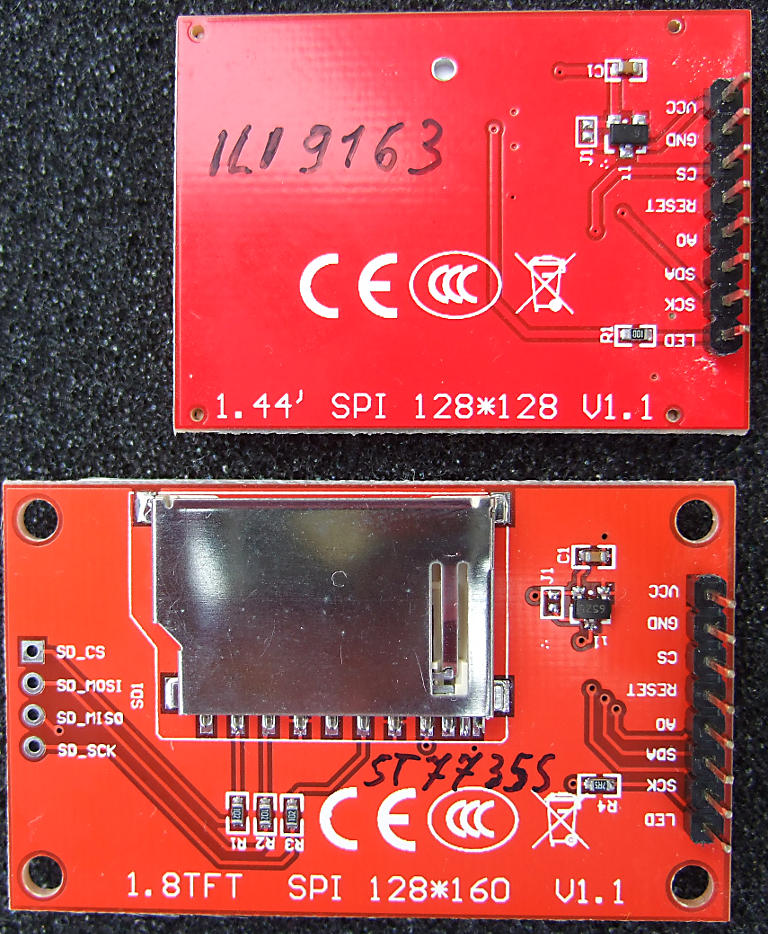
\includegraphics[width=8cm]{../PNG/Color_ILI9163_ST7735.jpg}
\caption{Rückseite der beiden Color-LCD's}
\label{fig:Color_both}
\end{figure}

Das 128x128 Pixel Modul benutzt einen ILI9163 Kontroller.
Das 128x160 Pixel Modul benutzt einen sehr ähnlichen ST7735 Kontroller.
Getestet habe ich die Module mit einem Adapterboard, der die Verbindungen
der SPI-Signale und der Stromversorgung zu der Anschlußleiste des normalen Textdisplays
herstellt. Die Anpassung der \(5V\) Signale des ATmega an die \(3.3V\) Eingänge des Kontrollers
habe ich mit seriellen \(10k\Omega\) Widerständen vorgenommen.
Die Hintergrundbeleuchtung (LED) ist für diese Module unbedingt erforderlich, da sonst
nichts erkennbar ist.
Aufgrund der hohen Pixelzahl in vertikaler Richtung können auf den Displays mehr Textzeilen dargestellt
werden. Für das 128x128 Pixel Display können bis zu 8 Textzeilen mit einem 12x8 Font dargestellt werden,
Für das 128x160 Pixel Display sind es sogar 10 Textzeilen.
Auf dem Foto \ref{fig:Color_PNP} ist das Ergebnis einer Messung eines Germanium Transistors auf einem
128x128 Pixel Display zu sehen.

\begin{figure}[H]
\centering
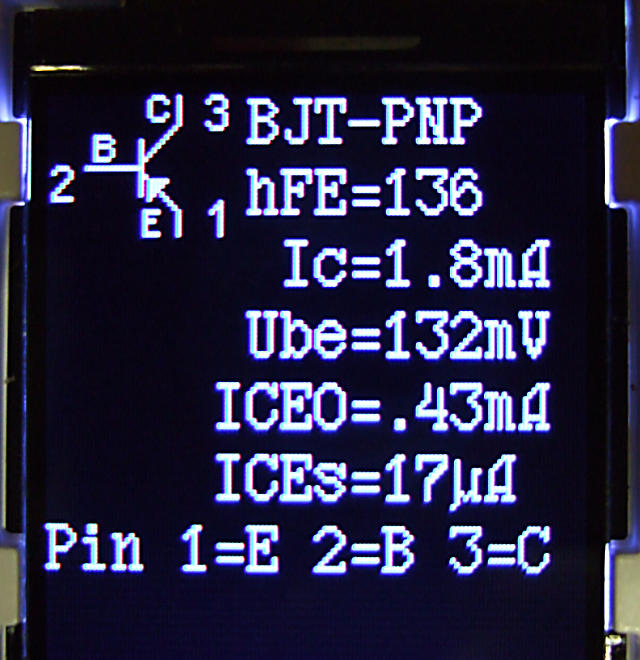
\includegraphics[width=8cm]{../PNG/Color_PNP_ILI9163.jpg}
\caption{Messung eines bipolaren PNP Transistors}
\label{fig:Color_PNP}
\end{figure}

Die Farbmöglichkeiten der Displays werden derzeit nicht genutzt. Lediglich die Hintergrundfarbe
und die Vordergrundfarbe könnten in der Datei lcd\_defines.h oder in der Makefile verändert werden.
Es wird das 16-Bit Farbmodell der Kontroller benutzt, die Vordergrundfarbe kann mit der Konstanten
LCD\_FG\_COLOR und die Hintergrundfarbe mit der Konstanten LCD\_BG\_COLOR eingestellt werden.

\section{Hinweise für den Aufbau des TransistorTesters}
Jede LCD-Anzeige-Einheit mit mindestens 2x16 Zeichen und einem HD44780-kompatiblen Controller kann mit
dem TransistorTester benutzt werden.
Man sollte auf den Strombedarf der Hintergrundbeleuchtung achten, einige Anzeigen benötigen
mehr Strom als andere.
Ich habe OLED-Anzeigen ausprobiert, aber diese Anzeigen haben teilweise die Messung des
ATmega beeinflusst und werden nicht empfohlen. Auch das Laden der Spezialzeichen für die 
Widerstandsdarstellung hat mit OLED's Schwierigkeiten ergeben.

Die Widerstände R1 bis R6 sind kritisch für die Messungen und diese \(680\Omega\) und
\(470k\Omega\) Widerstände sollten Messwiderstände sein (Toleranz von \(0,1\%\)), um 
die volle Genauigkeit zu erreichen.
Man sollte Präzisions-Sockel für den ATmega-Mikrocontroller verwenden, um
die Austauschbarkeit des Mikrocontrollers sicherzustellen.
Es kann ein ATmega8, ATmega168 und ATmega328 Mikrocontroller verwendet werden.
Empfohlen wird ein ATmega328, wenn man alle Funktionen nutzen möchte.

Jedenfalls sollte man zuerst alle Bauteile ohne den Mikrocontroller bestücken.
Es wird als IC2 ein moderner ,,low voltage drop''-Spannungsregler wie MCP1702-5002 empfohlen, weil
dieser nur \(2\mu A\) Ruhestrom benötigt und auch noch \(5V\) liefern kann, 
 wenn die Eingangsspannung nur \(5,4V\) beträgt.
Aber dieser Regler ist leider nicht Pin-kompatibel zum bekannteren 78L05-Regler im TO-92-Gehäuse!

Nachdem alle benötigten Bauteile bestückt sind, sollte zuerst die Batterie
oder das Netzteil angeschlossen werden. Das LCD sollte dabei nicht angeschlossen sein, und der Mikrocontroller sich noch nicht im Sockel befinden.
Man sollte die Betriebsspannung des Mikrocontrollers und der LCD-Anzeige
überprüfen während der Start-Taster gedrückt wird.
Die Betriebsspannung sollte verschwinden, wenn man den Start-Taster loslässt.
Wenn die Betriebsspannung die richtige Polarität und Grösse hatte,
sollte man die Strom-Versorgung entfernen und den Mikrocontroller 
richtig herum einstecken. Seien Sie bitte vorsichtig und stellen Sie sicher,
dass alle Pinne des Mikrocontrollers im Sockel stecken.
Danach können Sie das LCD anschliessen. Prüfen Sie, dass die GND- und VCC-Anschlüsse des LCD richtig mit der Baugruppe verbunden sind.

Wenn Sie sicher sind, dass alles richtig angeschlossen ist, schliessen Sie
die Spannungsversorgung wieder an.
Wenn Sie den ATmega schon programmiert haben, können Sie den Start-Taster
drücken.
Durch das Drücken des Start-Tasters sollte die Hintergrundbeleuchtung
der LCD-Anzeige angehen.
Wenn Sie den Taster loslassen, sollte die LED auf der Platine schwach leuchten.
Beachte, dass die Software für den Mikrocontroller für den richtigen
Prozessor-Typ übersetzt sein muss. Ein Programm für den ATmega8 läuft
nicht auf einem ATmega168!

\section{Umrüstung von Tester Versionen nach Markus F.}
\label{sec:change_markus}
\begin{description}

\item[Spannungsüberwachung]  
Das Problem zeigt sich durch sofortiges Abschalten beim Einschaltversuch.
Bei den von mir empfohlenen Einstellungen der fuses (Makefile) wird die Spannungsüberwachung der
verschiedenen ATmega-Versionen auf \(4V\) gesetzt (brown out level). Deswegen kann es beim
Einschalten des Testers zu Problemen kommen, weil der Pin PD6 versucht, den \(100nF\)-Kondensator C2
direkt zu schalten. Dabei kann es zu einem unerwünschten \(5V\) Spannungseinbruch kommen.
Der Kondensator C2 kann problemlos auf \textless~\(10nF\) verkleinert werden. Nach Möglichkeit sollte
man statt der direkten Verbindung PD6 zum Kondensator einen Widerstand \textgreater~\(220\Omega\) 
als Verbindung benutzen.
\item[Verbessern des Einschaltverhaltens]
Der Fehler zeigt sich oft, dass der Tester bei gedrücktem Taster zwar einschaltet, aber wieder
abschaltet, wenn der Taster losgelassen wird. Das Problem tritt öfter auf, wenn die Hintergrund-
Beleuchtung des LCD viel Strom braucht.
Der Widerstand R7 zur Basis des PNP-Transistors T3 war mit \(27k\Omega\) sehr auf Stromsparen
optimiert. Der Widerstand sollte besser auf \(3,3k\Omega\) verkleinert werden um auch bei
geringerer Batteriespannung oder bei geringem Stromverstärkungsfaktor des PNP-Transistors T3
ein sicheres Einschalten zu gewährleisten.
\item[Zusätzlicher Pull-Up-Widerstand an PD7]
Der Fehler zeigt sich dadurch, dass der Tester nach einer kurzen Anzeigezeit mit der Meldung
,,Timeout'' abschaltet. Die Software ist standardmäßig so konfiguriert (Option PULLUP\_DISABLE),
dass die internen Pull-Up-Widerstände abgeschaltet sind.
Dadurch ist der Pegel am Pin PD7 nicht mehr definiert,
wenn er nicht durch den Taster oder T2 auf GND-Potential geschaltet ist. Ein externer
Pull-Up-Widerstand von \(27k\Omega\) nach VCC vermeidet diesen Fehler.
\item[Kondensator C1 am AREF Pin]
In vielen Entwürfen wird hier ein \(100nF\)-Kondensator verwendet, so auch im Entwurf vom Markus Frejek.
Solange die Referenzspannung des ADC nicht verändert wird, ist das auch in Ordnung.
Bei der Software für den Transistortester für den ATmega168/328 wird aber eine automatische
Umschaltung der Referenzspannung von \(5V\) auf die interne Referenzspannung von \(1,1V\) vorgenommen,
wenn die Eingangsspannung unter etwa \(1V\) liegt. Damit wird eine bessere Auflösung erreicht.
Leider erfolgt die Umschaltung von \(5V\) auf die \(1.1V\) sehr langsam, was eine zusätzliche
Wartezeit von \(10ms\) erfordert. Durch den Austausch des \(100nF\) Kondensators gegen einen \(1nF\)
kann die Wartezeit deutlich verringert werden. Einen Einfluß des kleineren Kondensators
auf die Qualität der Messergebnisse habe ich nicht feststellen können. Selbst das Entfernen
des Kondensators hat keinen wesentlichen Einfluß. Wer den \(100nF\) Kondensator unbedingt
beibehalten möchte, kann die Makefile Option NO\_AREF\_CAP entfernen, um die längere
Wartezeit im Programm zu aktivieren.
\item[Nachrüsten eines \(8MHz\) Quarz]
Mit etwas Geschick kann auf der Lötseite der Platine ein \(8MHz\) Quarz direkt an PB6 und PB7
(Pin 9 und Pin 10) nachgerüstet werden.
Bei meiner Nachrüstung habe ich auf die beiden \(22pF\)-Kondensatoren verzichtet.
Bei allen eingesetzten Prozessoren hat diese Lösung problemlos funktioniert.
Aber die Nachrüstung ist nicht unbedingt erforderlich. Die Taktfrequenz sollte aber
wegen der besseren Zeitkonstanten-Auflösung  für die Kapazitäts-Messung auf jeden Fall \(8MHz\) betragen.
Die Frequenz \(8MHz\) ist auch bei RC-Oszillator-Betrieb durch Setzen der fuses möglich.
\item[Abblocken der Betriebsspannung]
Im Original-Schaltbild vom Markus F. ist nur ein \(100nF\)-Kondensator zum Abblocken der
VCC-Spannung (\(5V\)) eingezeichnet. Das ist deutlich zu wenig. Es sollte sowohl ein
\(100nF\) in unmittelbarer Nähe des ATmega als auch ein \(100nF\) in unmittelbarer Nähe
des Spannungsreglers vorhanden sein. Auch an den Eingang des Reglers gehört ein
100nF-Kondensator. Zusätzliche \(10\mu F\)-Kondensatoren (Elektrolyt oder Keramik) am Eingang und
Ausgang des Reglers können die Spannungsstabilität verbessern. Keramische \(10\mu F\)
Kondensatoren in SMD Bauform sind zum Nachrüsten meist besser geeignet und
haben üblicherweise einen niedrigeren ESR-Wert.
\item[Auswahl des ATmega-Prozessors]
Die Grundfunktion des Testers ist immer noch mit dem ATmega8 möglich.
Dabei ist der Programmspeicher nahezu zu \(100\%\) benutzt.
Da die ATmega168 oder ATmega328 Prozessoren pinkompatibel zum ATmega8 sind,
kann der Austausch nur empfohlen werden. Mittlerweile sind die Preise für
den ATmega328 so günstig, dass eigentlich nichts mehr für den ATmega168 spricht.
Mit dem ATmega168/328 gewinnt man folgende Vorteile:
Selbsttestfunktion mit automatischem Abgleich.\\
Erhöhung der Messgenauigkeit durch automatische Umschaltung der ADC-Referenzspannung.\\
Messung von Induktivitäten, deren Widerstandswert \textless~\(2100\Omega\) ist.\\
Messung des ESR-Wertes von Kondensatoren \textgreater~\(20nF\).\\
Die Auflösung der Widerstandsmessung unter \(10\Omega\) beträgt \(0,01\Omega\).\\
Der PC3-Pin kann für eine serielle Ausgabe genutzt werden.
\item[Fehlende Präzisionsreferenz]
Normalerweise sollte die fehlende Präzisionsreferenz auch bei unbeschaltetem PC4-Pin
erkannt werden. In diesem Fall wird keine VCC=x.xV Anzeige in Zeile 2 beim Einschalten
angezeigt. Falls es zu der Anzeige kommen sollte, hilft ein nach VCC geschalteter 
\(2,2k\Omega\) Widerstand am PC4-Eingang.
\end{description}

\section{Chinesische Nachbauten mit Textdisplay}
Der Tester wird in China nach meinem Kenntnisstand in zwei Versionen mit Textdisplay nachgebaut.
Die erste Variante ist der Nachbau des ersten Entwurfs von Markus F. ohne ISP-Schnittstelle.
Der bestückte ATmega8 ist bei dieser Version gesockelt, kann also auch durch einen ATmega168/328 ausgetauscht werden.
Für diese Version gelten alle Hinweise des Unterkapitels \ref{sec:change_markus}.
Zusätzliche \(100nF\) keramische Kondensatoren sollten in der Nähe des ATmega an die VCC-GND und
AVCC-GND Anschlüsse zur besseren Spannungsstabilisierung angebracht werden.
Da auf der Platine ein ISP-Stecker fehlt, muß entweder ein ISP-Anschluß nachgerüstet werden oder
der Prozessor für die Programmierung ausgebaut werden.
Dabei muss beachtet werden, dass bei der Nachrüstung eines Quarzes der ISP-Programmer selbst
einen externen Takt zuführen muss, oder der Programmiersockel mit einem Quarz ausgerüstet sein muß.\\
Die zweite Variante ist weitgehend in SMD-Technik aufgebaut. Auch der ATmega168 oder ATmega328 
ist in einem 32TQFP Gehäuse fest verbaut.
Dafür ist ein 10-poliger ISP-Stecker für die Programmierung auf der Platine vorgesehen.
Ich habe die Version ,,2.1 2012/11/06'' analysiert. Ein Fehler ist die Bestückung des Bauteils ,,D1'',
welches eigentlich die \(2,5V\) Präzisionsreferenz sein soll. Bestückt ist aber eine Zenerdiode.
Dieses Bauteil sollte entfernt werden. Hier kann eine Präzisionsreferenz wie LM4040AIZ2.5 oder
LT1004CZ-2.5 angeschlossen werden. Eine fehlende Präzisionsreferenz wird von der Software erkannt,
so dass sie nicht unbedingt erforderlich ist.
Bei meinem Exemplar war die Software Version 1.02k installiert. Der 10-polige ISP-Stecker war nicht
bestückt und ich musste zusätzlich eine Brücke von Pin 10 nach Pin 6 nachlöten. Mein Programmer hat eine 
GND-Verbindung an Pin 10 erwartet, der Tester hatte aber nur bei Pin 4 und Pin 6 eine GND-Verbindung.
Die Beschriftung des ATmega168 war abgeschliffen und es gab keine Dokumentation zum Gerät.
Die Sicherheits-Bits des ATmega waren gesetzt, sodass sich das Programm nicht auslesen ließ.
Ich konnte aber problemlos die Software Version 1.05k installieren.
Die gleiche Softwareversion 1.05k hat bei einem anderen Nutzer mit der China-Version ,,2.2 2012/11/26'' Probleme
gemacht. Die Software 1.05k lief hier erst, als ein weiterer \(100nF\) SMD Kondensator zwischen die Pins 18-AVCC
und 21-GND ergänzt wurde. Die Software 1.05k benutzt bei Wartezeiten den Schlafzustand des ATmega.
Deswegen wechselt der Strombedarf häufiger und der Spannungsregler wird mehr beansprucht.
Aufgefallen ist mir weiter, dass die VCC-Spannung mit einem \(100nF\) keramischen Kondensator und mit
einem \(220\mu F\) elektrolytischen Kondensator in der Nähe des 78L05-Spannungsreglers abgeblockt ist.
Die \(9V\) Spannungszufuhr ist mit den gleichen Kondensatoren abgeblockt, allerdings am Emitter des PNP-Transistor
(parallel zur Batterie), nicht direkt am Reglereingang.
Die Leiterbahnen vom ATmega zu den Testports sind teilweise sehr dünn, sodass ich einen Widerstand
von etwa \(100m\Omega\) pro Signalweg messen konnte. Dies ist wohl mit der Grund dafür, dass zwei
mit \(0\Omega\) verbundene Pinne einen Widerstandswert von \(0,3\Omega\) messen.
Bei der ESR-Messung kann dies normalerweise durch den Nullabgleich kompensiert werden.
Bei der Messung von Widerständen unter \(10\Omega\) werden die im Selbsttest ermittelten Offsets 
ab der Softwareversion 1.07k berücksichtigt.

\section{Chinesische Nachbauten mit graphischem Display}
Neuere Nachbauten verwenden ein 128x64 Pixel graphisches Display wie zum Beispiel eine Version von Fish8840.
Bei dieser Version wird eine veränderte Schaltung für das Einschalten benutzt. Die Abbildung \ref{fig:Fish8840}
zeigt einen Ausschnitt der Schaltung.

\begin{figure}[H]
\centering

\includegraphics[width=12cm]{../FIG/Fish8840.eps}
\caption{Ausschnitt aus der Schaltung von Fish8840}
\label{fig:Fish8840}
\end{figure}

Wie an den Widerständen R8 und R15 zu erkennen ist, 
wird mit 2:1 ein anderes Teilerverhältnis für die Batteriespannung wie im Original verwendet.
Außerdem ist R15 direkt an die Batterie angeschlossen, was zu einem geringen Stromverbrauch im
ausgeschalteten Zustand führt. Hier sollte R15 besser an das Drain von Q1 beziehungsweise an den
Eingang des Spannungsreglers angeschlossen werden um den unnötigen Batterieverbrauch zu vermeiden.
Eine entsprechende Änderung auf der Platine zeigt die Abbildung \ref{fig:Fish8840patch}.
Eine Leiterbahn ist zwischen R17 und D5 getrennt und mit einem Stück Kupferlackdraht eine
neue Verbindung zwischen Q1 und R15 gelötet.

\begin{figure}[H]
\centering
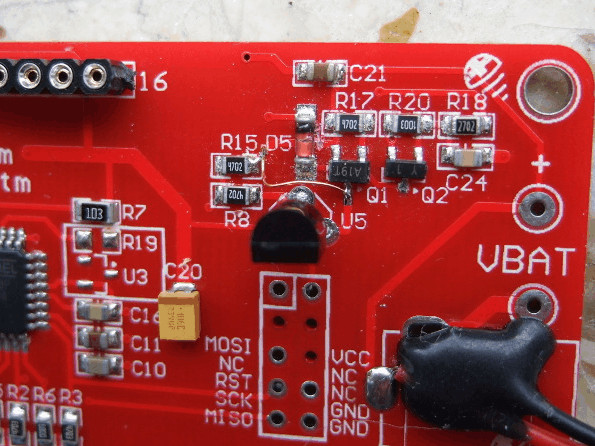
\includegraphics[width=12cm]{../PNG/Fish8840patch.jpg}
\caption{Foto der geänderten Fish8840 Platine}
\label{fig:Fish8840patch}
\end{figure}

Das Verhältnis des Spannungsteilers muss bei der Konfiguration in der Makefile auf jeden Fall angegeben
werden bevor eine Software aufgespielt wird (z.B. mit BAT\_NUMERATOR=66).

Das Display Module des Fish8840 Testers besitzt einen \(3.3V\) Spannungsregler, der die Betriebsspannung
des Display-Controllers anpassen soll.
Da es über die Datenleitungen des Display-Moduls zu einer Erhöhung der \(3.3V\) Betriebsspannung wegen
der \(5V\) Signale vom ATmega kommt,
wird eine Adapterschaltung nach Abbildung \ref{fig:Fish8840Adapt} empfohlen. Hier sind in die vier
Datenleitungen vier serielle Widerstände mit jeweils \(2.7k\Omega\) auf einer kleinen Lochrasterplatine
zwischengeschaltet.
Längere Gewindebolzen müssen nun verwendet werden, um das Display mit der Adapterplatine auf dem
Fish8840 Tester zu befestigen.

\begin{figure}[H]
  \begin{subfigure}[b]{9cm}
    \centering
    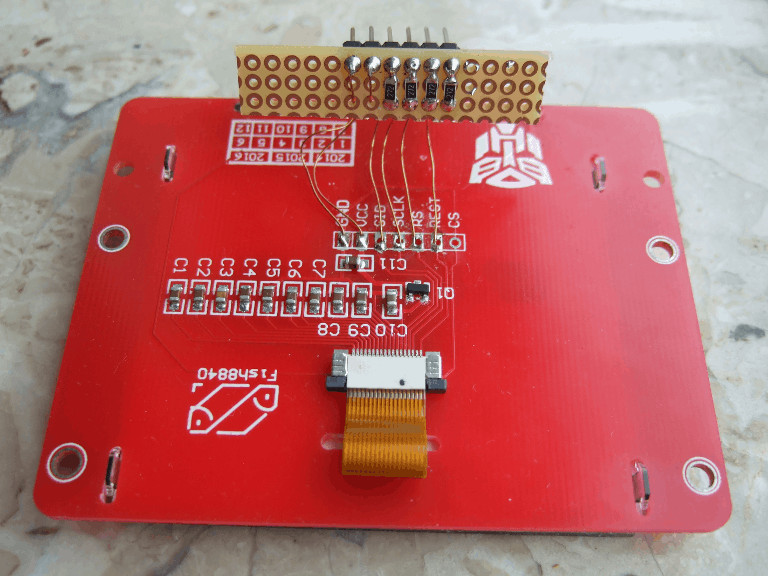
\includegraphics[width=9cm]{../PNG/Fish8840Adapt1.jpg}
    \caption{Display mit Adapter}
  \end{subfigure}
  ~
  \begin{subfigure}[b]{9cm}
    \centering
    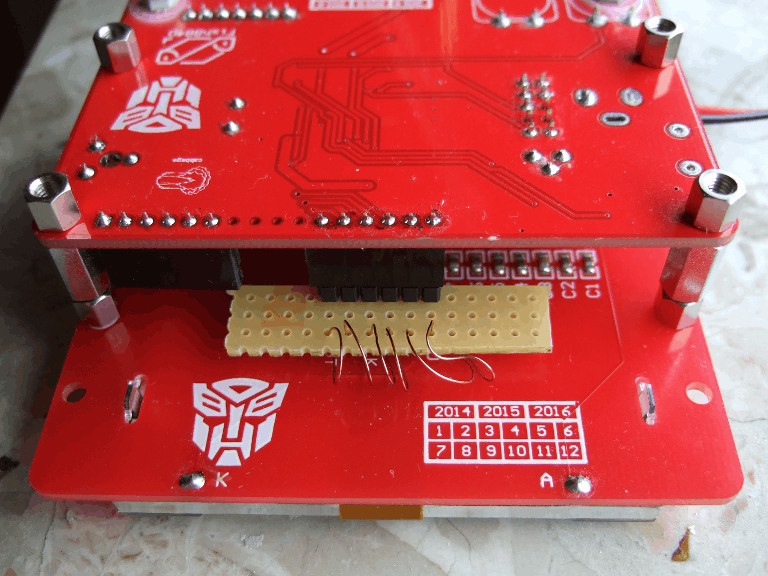
\includegraphics[width=9cm]{../PNG/Fish8840Adapt2.jpg}
    \caption{Fertig montierter Tester}
  \end{subfigure}
  \caption{Adapter für einen korrekten Display Anschluß}
  \label{fig:Fish8840Adapt}
\end{figure}

Anstelle dieser Umrüstung kann mit der Makefile Option LCD\_SPI\_OPEN\_COL auch eine spezielle Ausgangsschaltung
der 4~SPI Signale des ATmega benutzt werden.
Dabei werden die Ausgänge nicht auf VCC Pegel geschaltet,
sondern nur die internen ,,Pull-Up'' Widerstände während der Ausgabe für den high Pegel freigeschaltet.
Wenn die Option PULLUP\_DISABLE gesetzt ist, ist ein externer Pull-Up Widerstand für das
Reset Signal (PD0) erforderlich.
Weil die Datensignale nie direkt auf VCC geschaltet werden, kann die \(3.3V\) Versorgung des LCD-Controllers
auch nicht überhöht werden.
Die mir vorliegende Platine des Fish8840 Testers hat alle Signale für den Anschluß eines
Textdisplays an die LCD-Steckerleiste geführt. 
Deshalb kann die Platine auch mit einem Textdisplay umgerüstet werden, wenn die Buchsenleiste
ergänzt wird und das Potentiometer für die Kontrasteinstellung nachgerüstet wird.
Der Versorgungspin 15 für die Hindergrundbeleuchtung ist allerdings direkt mit VCC verbunden.
Bei einer Installation eines Textdisplays sollte darauf geachtet werden, daß auf dem Displaymodul
ein serieller Widerstand zur LED vorhanden ist.
Selbstverständlich muß die Software für eine andere Displayversion angepasst werden.
Auch die Erweiterungsmöglichkeiten des Testers sind bei der Fish8840 Platine möglich.\\

Für die Funktionsfähigkeit kann natürlich keine Gewähr gegeben werden.
Leider kann der Originalzustand der chinesischen Software-Variante auch nicht gesichert werden,
da die Sicherheits-Bits des ATmega328 gesetzt sind.
Es gibt also keinen Weg zurück zur Originalversion der Software.\\ 

Eine weitere Version mit graphischem Display ist die WEI\_M8 Platine, die in Abbildung \ref{fig:WeiM8}.
Dieser Nachbau benutzt als Stromquelle einen LiIon Akkumulator im AA (Mignon) Format, der über
eine Micro-USB Schnittstelle geladen werden kann. Ein Betrieb ohne Akku ist über die USB-Schnittstelle
ebenfalls möglich.

\begin{figure}[H]
\centering
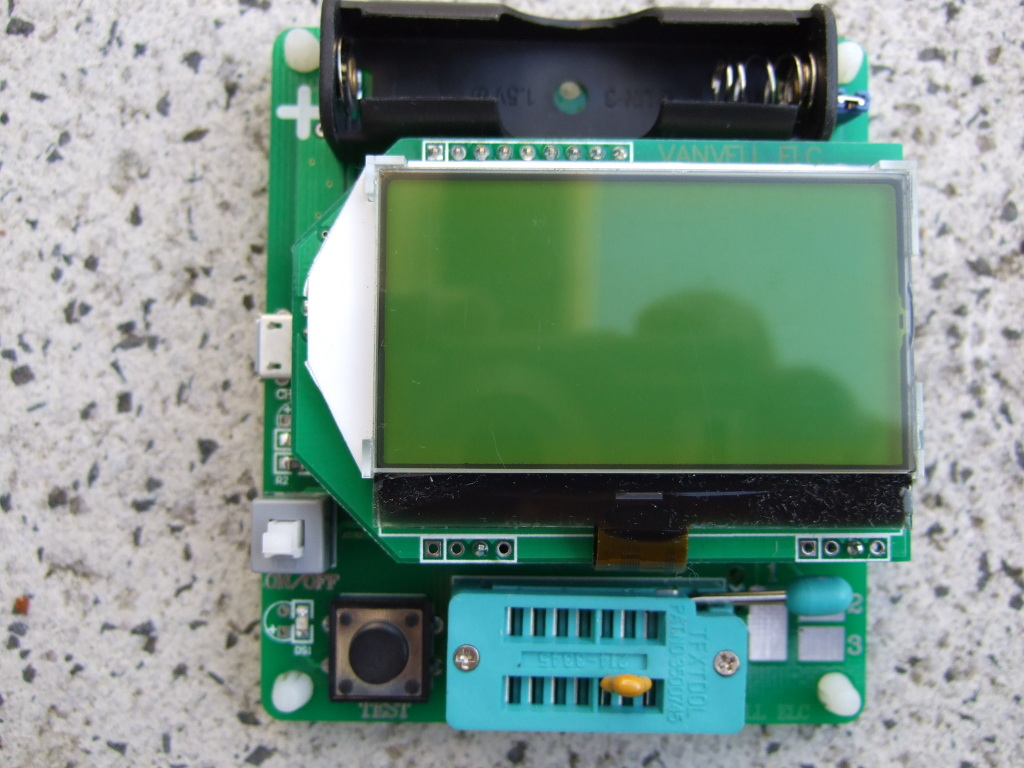
\includegraphics[width=12cm]{../PNG/WEI_M8.JPG}
\caption{Foto des chinesischen WEI\_M8 Testers}
\label{fig:WeiM8}
\end{figure}

Erfreulich ist, dass für die Signalleitungen des Displays serielle Widerstände
auf der Adapterplatine vorgesehen sind, wie in der linken Abbildung von~\ref{fig:WeiM8int}
zu sehen ist. Damit ist eine Überhöhung der \(3.3V\) Versorgung für den Displaycontroller
wegen der \(5V\) Signalpegel vom ATmega nicht zu befürchten.

\begin{figure}[H]
  \begin{subfigure}[b]{9cm}
    \centering
    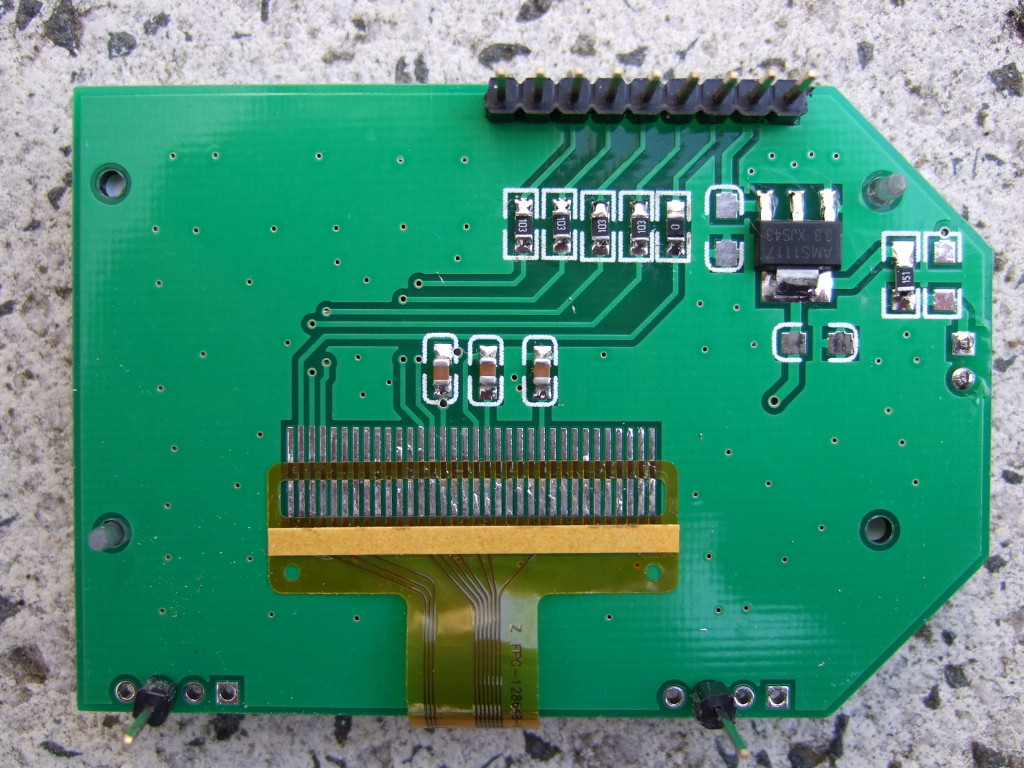
\includegraphics[width=9cm]{../PNG/WEI_M8_D.JPG}
    \caption{Adapterplatine für das Display}
  \end{subfigure}
  ~
  \begin{subfigure}[b]{9cm}
    \centering
    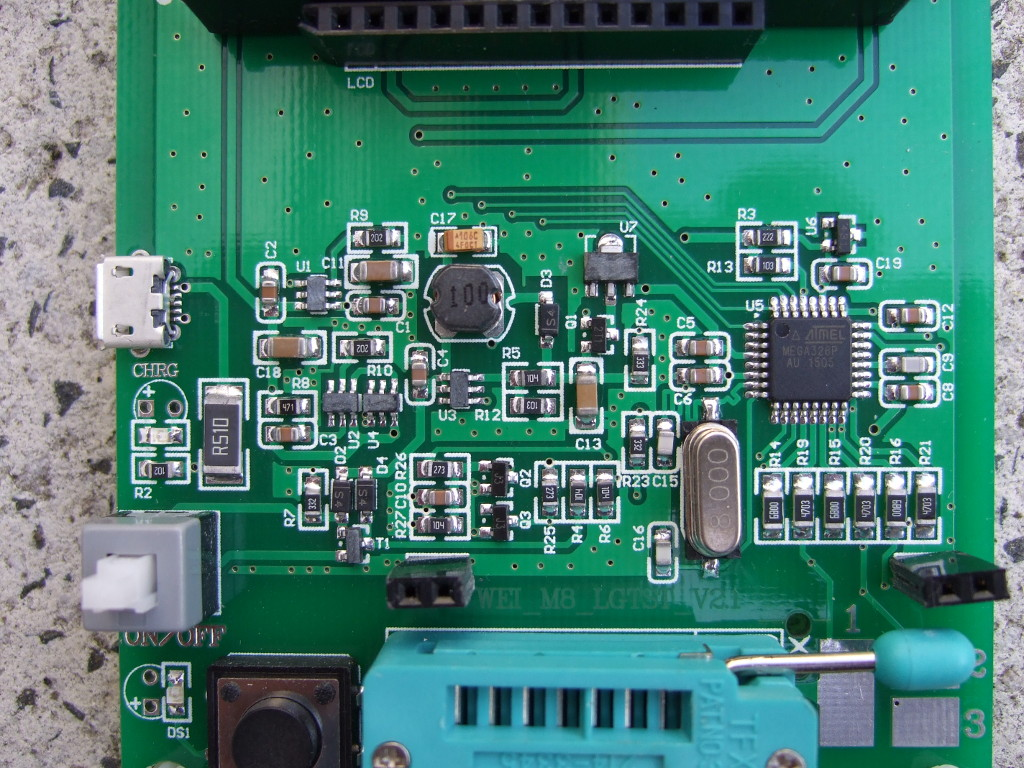
\includegraphics[width=9cm]{../PNG/WEI_M8_L.JPG}
    \caption{Grundplatine}
  \end{subfigure}
  \caption{Innenleben des WEI\_M8 Testers}
  \label{fig:WeiM8int}
\end{figure}


Bei der Aufrüstung auf die 1.12k Version
der Software ergaben sich einige Schwierigkeiten. Wenn die extended Fuse wie empfohlen auf
0x04 (oder 0xfc) gesetzt wird, kam es bei bestimmten Messungen zu ,,Brown Out'' Resets des
Prozessors. Diese Resets werden durch kurzzeitige Spannungseinbrüche der VCC Versorgung
verursacht. Die Platine wurde deshalb mit einem \(4.7\mu F\) kermamischen Kondensator
am Eingang des Spannungsreglers und mit einem \(10\mu F\) keramischen Kondensator am
Reglerausgang (VCC) zusätzlich abgeblockt. Sowohl vor der Nachrüstung als auch danach
wurde bei bipolaren Transistoren ein Kollektor-Reststrom (ICEO oder ICEs) gemessen.
Erst der Austausch des LDO-Spannungsreglers (unbekannter Typ) durch einen MCP1702-5002
brachte hier Abhilfe. Die Abbildung \ref{fig:WeiM8mod} zeigt die umgerüstete Platine
mit den schräg montierten nachgerüsteten Kondensatoren und dem MCP1702 Regler.
Wer die Kondensatoren nicht nachrüsten möchte, sollte die extended Fuse auf 0x07 (0xff)
setzen, damit ein Betrieb möglich ist. Damit bleiben die Spannungseinbrüche unentdeckt.

\begin{figure}[H]
\centering
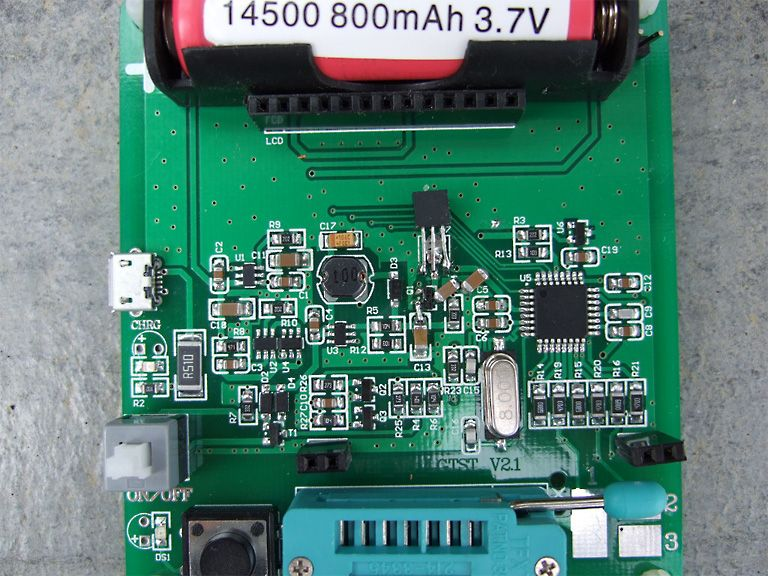
\includegraphics[width=12cm]{../PNG/WEI_M8_modified.JPG}
\caption{Foto des umgerüsteten WEI\_M8 Testers}
\label{fig:WeiM8mod}
\end{figure}

Eine weitere Version mit graphischem Display ist der LCD-T4 Tester mit einer gelben Platine.
Für das Aufspielen neuer Software habe ich das Display abgenommen.
Auf dem rechten Foto der Abbildung \ref{fig:T4_front} ist der Stecker für die ISP-Verbindung rechts oben
 neben den entsprechen Bohrungen der Platine in der richtigen Ausrichtung aufgelegt.
Für die Programmierung habe habe ich den Stecker nicht eingelötet, sondern nur eingesteckt und durch
seitlichen Druck mit einem Finger für die Dauer der Programmierung fixiert.
Dadurch kann der Stecker nach der Programmierung wieder leicht entfernt werden und das Display
an die ursprüngliche Stelle montiert werden.
Die Software 1.12k konnte übrigens problemlos aufgespielt werden.
Auch das Aktivieren der ,,Brown-Out'' Erkennung des Prozessors mit der extended fuse
brachte keine Überraschungen.

\begin{figure}[H]
  \begin{subfigure}[b]{9cm}
    \centering
    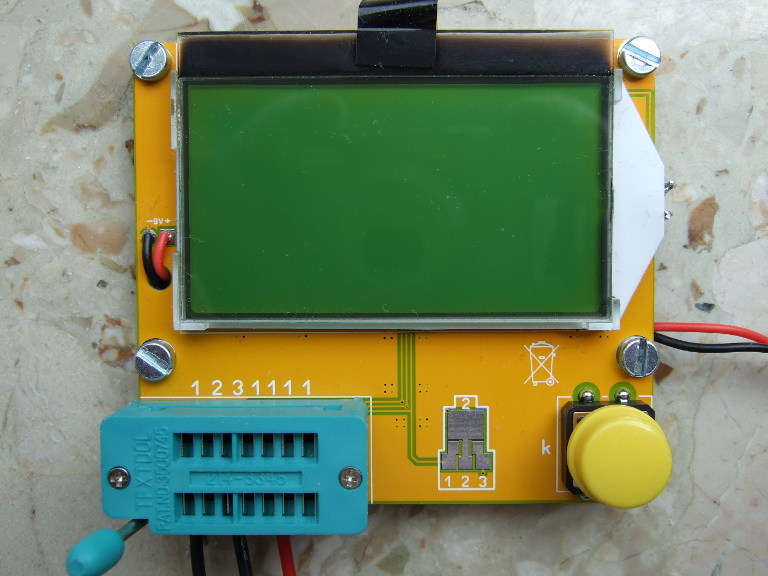
\includegraphics[width=9cm]{../PNG/T4_front.JPG}
    \caption{vollständig}
  \end{subfigure}
  ~
  \begin{subfigure}[b]{9cm}
    \centering
    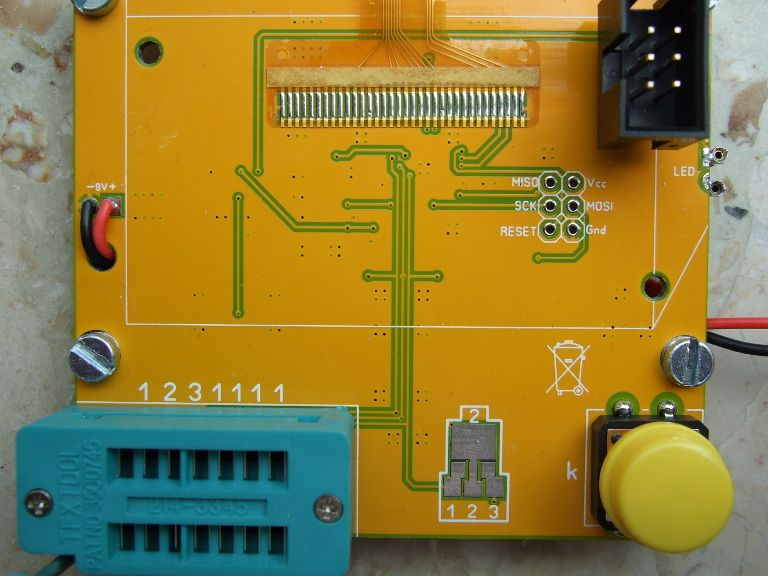
\includegraphics[width=9cm]{../PNG/T4_front_noLCD.JPG}
    \caption{mit abgenommenem Display}
  \end{subfigure}
  \caption{Frontansicht des T4 Testers}
  \label{fig:T4_front}
\end{figure}

Auf den Fotos der Rückseite in Abbildung \ref{fig:T4_back} sieht man die nachgerüsteten
\(5mm\) Gewindebolzen sowie die nachträglich angelöteten Kabel mit Messclips.
Da aber für die Datensignale des graphischen LCD-Controllers auch hier
keine Signalanpassung (\(5V~-\textgreater ~3.3V\)) erfolgt, ist das Setzen der Option LCD\_SPI\_OPEN\_COL ratsam.
Da die Nachrüstung eines ,,pull-up'' Widerstandes für das SPI-Reset Signal hier
aber schwierig durchzuführen ist, bleibt nur das Entfernen der Option
DISABLE\_PULLUP übrig. 
Für nachträgliche Erweiterungen ist diese Platine weniger geeignet, auch ein Austausch des
Displays ist hier nur schwer möglich.

\begin{figure}[H]
  \begin{subfigure}[b]{9cm}
    \centering
    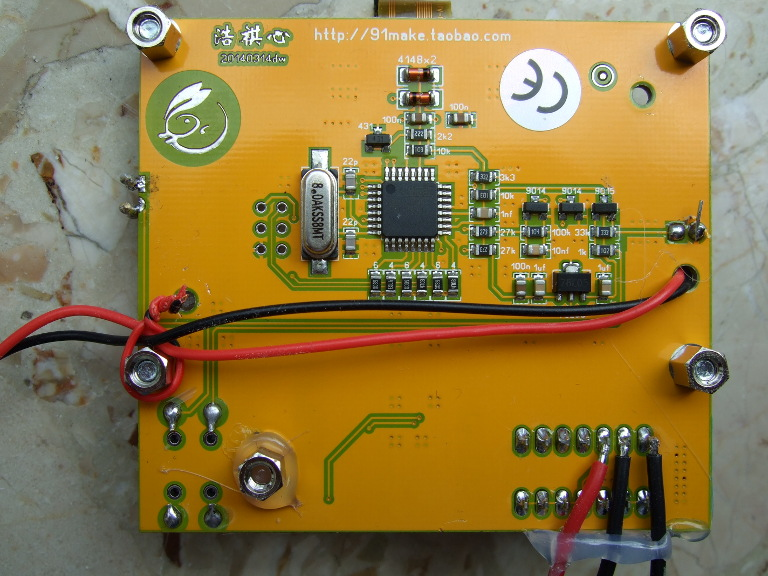
\includegraphics[width=9cm]{../PNG/T4_back.JPG}
    \caption{Bestückungsseite}
  \end{subfigure}
  ~
  \begin{subfigure}[b]{9cm}
    \centering
    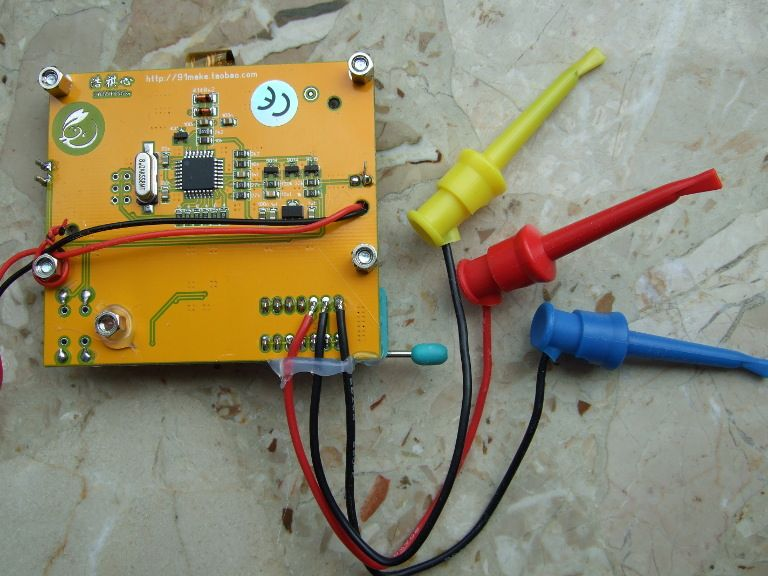
\includegraphics[width=9cm]{../PNG/T4_back_clips.JPG}
    \caption{mit Messkabeln}
  \end{subfigure}
  \caption{Rückansicht des T4 Testers}
  \label{fig:T4_back}
\end{figure}

Noch eine chinesische Version mit graphischem Display wird mit der Bezeichnung ,,GM328'' angeboten.
Bei dieser Version ist das graphische Display an eine 16-pol Buchsenleiste mit einer Tochterplatine
angeschlossen.
Dabei ist auch der Port PD5 über die Buchsenleiste Pin 6 an das CE (Chip Enable) Signal
des graphischen Controllers angeschlossen. Das CE Signal ist aber auf der Tochterplatine auch mit der
\(0V\) Power (GND) verbunden.
Das führt zu einem Kurzschluß, wenn der ATmega den PD5 Ausgang auf \(5V\) schalten möchte.
Neuere Versionen der Software schalten aber auch das CE Signal, auch wenn das Signal für den Betrieb nicht
benötigt wird.
Deswegen sollte bei dem ,,GM328'' Tester die Verbindung der Tochterplatine zum Pin 6 
der Anschlußleiste unterbrochen werden.

\section{Chinesische Bausätze mit Grafikdisplay}

Bisher sind zwei Bausätze mit grafischen Display und Drehimpulsgeber bekannt.
Der zuerst erschienene Bausatz verwendet ein Display mit ST7565 oder kompatiblen Controller (128x64 Pixel).
Außer dem Drehimpulsgeber ist  auch ein Eingang für die Frequenzmessung vorgesehen.
Für die Testports steht ein 14-poliger Textool Sockel, 3 Lötaugen für Kabel sowie ein Testpad
für SMD Bauteile zur Verfügung. 
Die Fotos~\ref{fig:Kit_mono} zeigen den zusammengebauten Bausatz.
Einer der beiden \(22 pF\) Kondensatoren 
wurde hier durch einen Trimmer auf der Lötseite ersetzt. Mit dem Trimmer läßt sich die Frequenz des Quarzes für genauere
Frequenzmessung bzw. Frequenzerzeugung abgleichen.

\begin{figure}[H]
  \begin{subfigure}[b]{9cm}
    \centering
    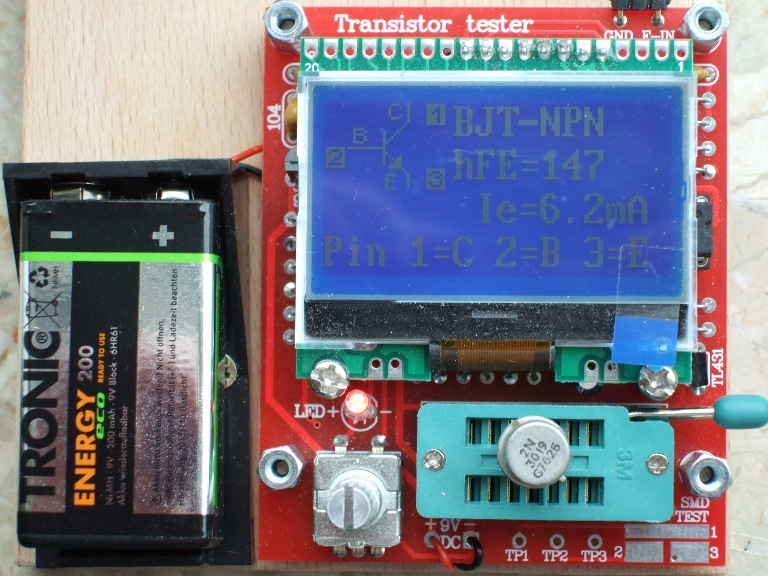
\includegraphics[width=9cm]{../PNG/Kit_ST7565a.jpg}
    \caption{zusammengebaut}
  \end{subfigure}
  ~
  \begin{subfigure}[b]{9cm}
    \centering
    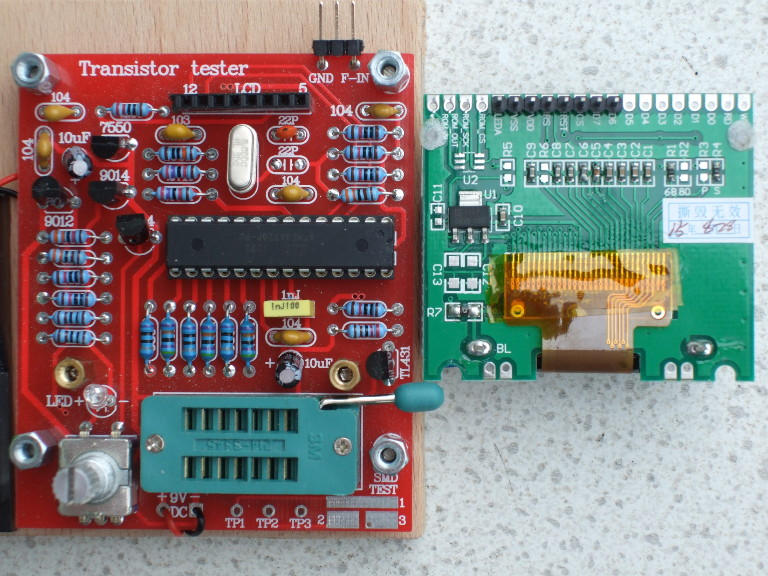
\includegraphics[width=9cm]{../PNG/Kit_ST7565b.jpg}
    \caption{mit abgenommenem Display}
  \end{subfigure}
  \caption{Bestückter Bausatz mit 128x64 Pixel Display}
  \label{fig:Kit_mono}
\end{figure}

Der später erschienene Bausatz verwendet ein Farbdisplay mit ST7735 Controller (128x160 Pixel) 
und hat zusätzlich zum Fequenzeingang noch einen Eingang für Spannungsmessung und einen Frequenzausgang.
Der Frequenzausgang ist aber nicht gepuffert, sondern ist lediglich zum Anschluß TP2 parallel 
angeschlossen. Bei der Spannungsmessung handelt es sich nur um die Messung einer positiven Gleichspannung bis 50V,
ein DC-DC Wandler für die Zenerspannungsmessung wurde nicht vorgesehen.
Die Fotos \ref{fig:Kit_color} zeigen den zusammengebauten Bausatz.
Auch hier wurde einer der beiden \(22 pF\) Kondensatoren 
wurde hier durch einen Trimmer (grün) ersetzt. 

\begin{figure}[H]
  \begin{subfigure}[b]{9cm}
    \centering
    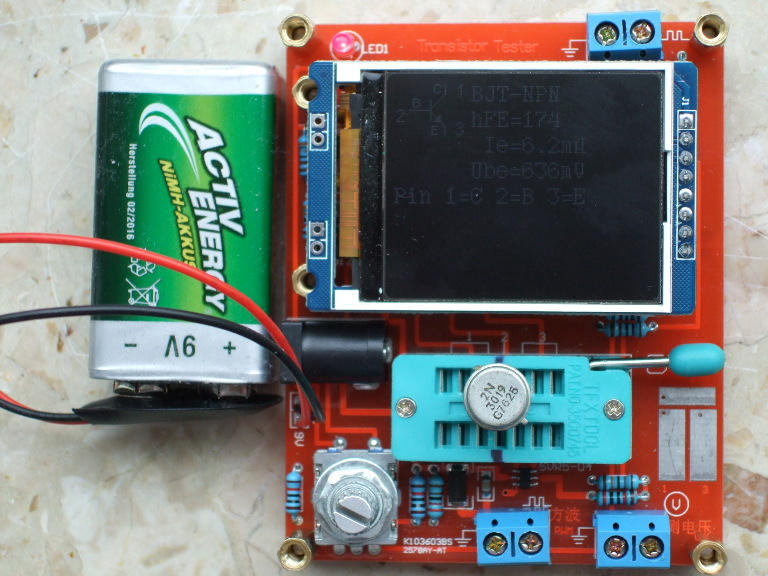
\includegraphics[width=9cm]{../PNG/Kit_Color_a.jpg}
    \caption{zusammengebaut}
  \end{subfigure}
  ~
  \begin{subfigure}[b]{9cm}
    \centering
    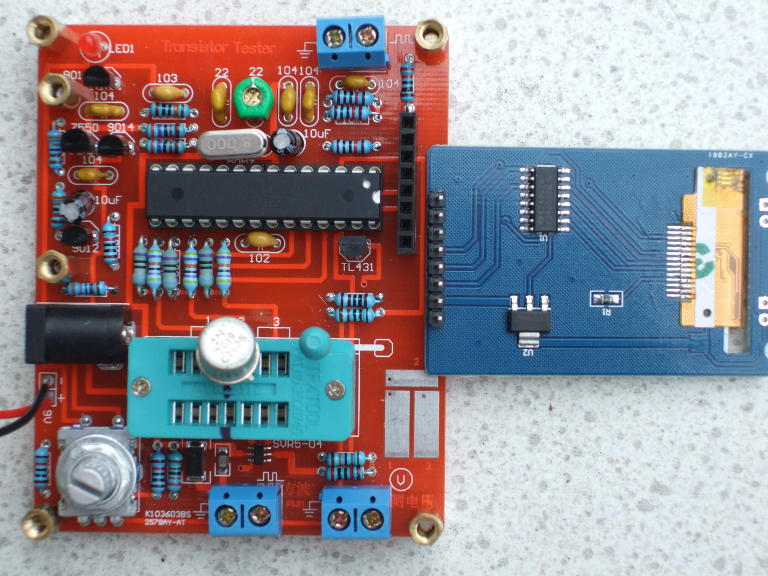
\includegraphics[width=9cm]{../PNG/Kit_Color_b.jpg}
    \caption{mit abgenommenem Display}
  \end{subfigure}
  \caption{Bestückter Bausatz mit 160x128 Pixel Farbdisplay}
  \label{fig:Kit_color}
\end{figure}

Beide Bausätze verwenden einen gesockelte DIP Version des ATmega328P und haben keinen 
ISP Stecker für das Aufspielen neuer Softwareversionen.
Die erste Version verwendet
ausschließlich bedrahtete Bauteile für die Hauptplatine. Die Meßwiderstände \(680\Omega\) und \(470k\Omega\)
waren bei meinem Bausatz mit einer 0.1\% Toleranz geliefert worden.
Selbst ein \(220 nF\) Kondensator für die Kalibration wurde bei diesem Bausatz mitgeliefert.
Der Bausatz mit dem Farbdisplay hat zusätzlich zum Anschluß für die 9V Batterie noch eine Buchse
für einen Netzteilanschluß. Die wenigen SMD-Bauteile waren schon auf der Platine bestückt,
so daß auch bei diesem Bausatz nur einfache Lötarbeiten durchzuführen sind.
Ein kleiner Nachteil der Version mit dem Farbdisplay ist die Geschwindigkeit der Ausgabe.
Speziell bei der Menübedienung fällt die deutlich langsamere Ausgabe negativ auf.
Andererseits hat das Farbdisplay eine deutlich höhere Pixelzahl und kann damit mehr Text darstellen. 
Beide Bausätze verwenden einen 3.3V Spannungsregler für die Versorgung der Display Controller auf
den vollständig bestückten Display-Platinen. Lediglich die Stiftleiste muß bei
der Displayplatine eingelötet werden.
Die Farbversion verwendet einen CD4050 Puffer für die Anpassung der Signalpegel.
Auf der Display-Platine der ST7565 Variante ist keine Anpassung der Signalpegel erkennbar.
Wahrscheinlich toleriert die gewählte Controller-Variante die 5V Signalpegel des ATmega328.
Es ist jedenfalls keine Schutzdiode gegen die 3.3V Versorgung bei diesem Controller feststellbar.

\section{Erweiterte Schaltung mit ATmega644 oder ATmega1284}

Eine erweiterte Schaltung für ATmega644/1284-Prozessoren wurde in Zusammenarbeit mit Nick L. aus
der Ukraine entwickelt. Die Schaltung nach Abbildung \ref{fig:t644tester} ermöglicht zusätzlich
einen Test von Quarzen und einen erweiterten Frequenzbereich für die Frequenzmessung.
Obwohl die Grundschaltung sehr ähnlich der Schaltung \ref{fig:ttester} ist, werden hier
andere Portbelegungen benutzt.
Ein Impulsdrehgeber nach Schaltung \ref{fig:RotExt} kann hier an PB5 und PB7 (statt PD1 und PD3) angeschlossen werden.
Beide Signale und auch die Versorgungssignale VCC und GND sind am ISP-Stecker verfügbar,
sodass die Erweiterung auch hier angeschlossen werden kann.\\

Der 16:1-Frequenzteiler 74HC4060 wird für höhere Frequenzen als \(2MHz\) immer benutzt.
Der Teiler kann aber auch für Frequenzen von \(25kHz\) bis \(400kHz\) benutzt werden, um mit der
Periodenmessung die Auflösung der Frequenzmessung zu verbessern.
Für die Umschaltung der Betriebszustände (Frequenzteiler und Quarz-Oszillator) werden
die Analogschalter 74HC4052 benutzt.
Die Tabelle \ref{tab:mega644-display} zeigt die Pinbelegung für den ATmega324/624/1284 Mikrocontroller für verschiedene Displayanschlüsse.
Die I\textsuperscript{2}C-Schnittstelle ist nur mit dem SSD1306-Controller möglich.
Die Signale der I\textsuperscript{2}C-Schnittstelle erfordern einen ,,Pull-Up''-Widerstand von etwa \(4,7k\Omega\) nach \(3,3V\).
Die Ausgänge des ATmega werden für die I\textsuperscript{2}C-Signale nur nach \(0V\) geschaltet.


\begin{table}[H]
  \begin{center}
    \begin{tabular}{| c || c | c | c | c |}
    \hline
      Port & Character LCD &  Graphik LCD & Graphik LCD  & Zusatzfunktion      \\
           &               &  SPI 4-Wire  &  I\textsuperscript{2}C         &                     \\
    \hline
    \hline
    PB2    &  LCD-RS         &            &             &       \\
    \hline
    PB3    &  LCD-E          & (LCD-CE)   &  LCD-SCL    &       \\
    \hline
    PB4    &  LCD-D4         & LCD-REST   &  LCD-SDA    &       \\
    \hline
    PB5    &  LCD-D5         & LCD-RS     &             & ISP-MOSI \\
           &                 &            &             & Drehgeber 2 \\
    \hline
    PB6    &  LCD-D6         & LCD-SCLK   &             & ISP-MISO \\
    \hline
    PB7    &  LCD-D7         & LCD-SI     &             & ISP-SCK  \\
           &                 &            &             & Drehgeber 1 \\
    \hline
    \end{tabular}
  \end{center}
  \caption{Verschiedene Varianten der Display-Anschlüsse}
  \label{tab:mega644-display}
\end{table}

Auch ein Display mit ST7108 Controller kann mit einer kleinen Zusatzschaltung an einen
ATmega644 oder ATmega1284 angeschlossen werden wie in der Abbildung~\ref{fig:ST7108lcd_644} gezeigt.
Bitte beachten Sie auch die verschiedenen Pinbelegungen der Displaymodule mit ST7108 Controller wie in
Tabelle~\ref{tab:ST7108types} auf Seite~\pageref{tab:ST7108types} angegeben.

\begin{figure}[H]
  \begin{subfigure}[b]{9cm}
    \centering
    
\includegraphics[width=8cm]{../FIG/ST7108serial164_644.eps}
    \caption{mit 74HCT164}
  \end{subfigure}
  ~
  \begin{subfigure}[b]{9cm}
    \centering
    
\includegraphics[width=8cm]{../FIG/ST7108serial595_644.eps}
    \caption{mit 74HCT595}
  \end{subfigure}
  \caption{Anschluss des ST7108 Controllers an einen ATmega644/1284}
  \label{fig:ST7108lcd_644}
\end{figure}



\begin{figure}[H]
\centering

\includegraphics[width=18cm]{../FIG/t644tester.eps}
\caption{Erweiterte Transistortester Schaltung mit ATmega644}
\label{fig:t644tester}
\end{figure}


\section{Aufbau mit ATmega1280 oder Arduino Mega}
Die Grundschaltung des Testers läßt sich auch mit einem Arduino Mega mit ATmega1280 oder
ATmega2560 als Shield aufbauen.
Die notwendigen Verbindungen zeigt die Abbildung~\ref{fig:t1280tester}.
Die Steckverbindungen des Arduino für die Datenverbindungen des Displays sind in güner Farbe eingezeichnet.
Die Bauteile mit roter Bezeichnung sind für die Funktion des Testers nicht erforderlich.
Der ATmega2560 Controller hat zwar viele Anschlußpins, aber nur ein einziger Pin hat die
erforderlichen Verbindungen für beide Methoden der Frequenzmessung. 
Der Anschlußpin muß als Takteingang für einen Zähler geschaltet werden können und außerdem muß
der Pin ein Unterbrechungssignal (Interrupt) bei Pegelwechsel erzeugen können.
Dies ist nur für den Pin PE6 (T3/INT6) der Fall. Die anderen Takteingänge der Zähler
PD7 (T0), PD6 (T1), PH7 (T4) und PL2 (T5) können nicht für die Erzeugung des Unterbrechungssignals
bei Pegelwechsel verwendet werden.
Leider ist der PE6 Pin nicht mit den Steckerleisten des Arduino verbunden.
Der PE5 Pin (7) ist mit dem Anschluß 3 der PWM Buchsenleiste des Arduino verbunden und kann
am Atmega2560 mit dem PE6 Pin (8) gebrückt werden.
Der Ausgang der Frequenzerzeugung ist am Pin PB6 (OC1B) verfügbar. Dieser Pin ist mit Anschluß 12
der PWM-Buchsenleiste verbunden.
Auf den ISP-Stecker kann für den Arduino verzichtet werden, da das Programm über
das USB-Interface und den Bootloader geladen werden kann.  Mit dem
Bootloader gibt es lediglich eine kleine Verzögerung des Programmstarts.

\begin{figure}[H]
\centering

\includegraphics[width=18cm]{../FIG/t1280tester.eps}
\caption{Transistortester Schaltung mit ATmega1280, ATmega2560 oder Arduino Mega}
\label{fig:t1280tester}
\end{figure}

Natürlich können alle unterstützten Displays auch an die ATmega1280 oder ATmega2560 angeschlossen
werden, wie in der Tabelle~\ref{tab:display-1280} angegeben.

\begin{table}[H]
  \begin{center}
    \begin{tabular}{| c || c | c | c | c | c | c |}
    \hline
           & Character     &  ST7565     & ST7920       & ST7108       & SSD1306     & Zusatzfunktion \\
      Port & LCD           &    SPI      & seriell      & seriell      &    I\textsuperscript{2}C      & \\
    \hline
    \hline
    PA0    &  LCD-D4       &   LCD-REST  &  LCD-RESET   & HC595-RCK       &             & \\
    \hline
    PA1    &  LCD-D5       &   LCD-RS    &              & LCD-CS2        &             & Drehgeber-2 \\
    \hline
    PA2    &  LCD-D6       &   LCD-SCLK  &              & HC164-CLK      &             & \\
    \hline
    PA3    &  LCD-D7       &   LCD-SI    &              & LCD-CS1        &             & Drehgeber-1 \\
    \hline
    PA4    &  LCD-RS       &             &   LCD-B0     & LCD-RS         &   LCD-SDA   & \\
           &               &             &              & HC164-SER      &             & \\
    \hline
    PA5    &  LCD-E        &  (LCD-CE)   &   LCD-EN     & LCD-EN         &   LCD-SCL  & \\
    \hline
    PA7    &  Tastensignal &             &              &                &             & \\
    \hline
    \end{tabular}
  \end{center}
  \caption{Pinbelegungen für verschiede Displays an ATmega1280/2560}
  \label{tab:display-1280}
\end{table}


\section{Programmierung des Mikrocontrollers}
Ich gebe die Software für den Mikrocontroller in Quelltext heraus.
Die Entwicklung wurde mit dem Linux-Betriebssystem (Ubuntu bzw. Mint) gemacht
und wird gesteuert mit einer Makefile.
Die Makefile stellt sicher, dass die Software entsprechend der vorher in der Makefile 
eingestellten Optionen übersetzt wird. Schauen Sie bitte in die Datei LiesMich.txt
im Verzeichnis trunk/default und in das Konfigurations-Kapitel~\ref{sec:config} ab Seite~\pageref{sec:config}.
Das Ergebnis der Übersetzung hat die Dateierweiterung .hex und .eep.
Üblicherweise heißen die Dateien TransistorTester.hex und TransistorTester.eep .
Die .hex-Datei enthält die Daten für den Programmspeicher (Flash) des ATmega-Prozessors.
Die .eep-Datei enthält die Daten für den EEPROM des ATmega.
Beide Dateien müssen in den richtigen Speicher geladen werden.

Zusätzlich muss der ATmega mit den ,,fuses'' richtig konfiguriert werden.
Wenn Sie meine Makefile zusammen mit dem Programm avrdude \cite{avrdude} benutzen, brauchen Sie
keine genaue Kenntnis über die Einzelheiten der fuses.
Sie brauchen nur ,,make fuses'' aufrufen, wenn Sie keinen Quarz benutzen oder Sie
müssen ,,make fuses-crystal'' aufrufen, wenn Sie einen \(8MHz\) Quarz auf der Baugruppe installiert haben.
Bei der ATmega168-Serie der Mikrocontroller können Sie alternativ auch
,,make fuses-crystal-lp'' aufrufen für den low power Quarz-Betrieb.
Benutzen Sie niemals die Quarz-Variante, wenn Sie keinen \(8MHz\) Quarz installiert haben.
Wenn Sie sich nicht sicher mit den fuses sind, lassen Sie diese erst einmal wie
vom Werk gesetzt und bringen Sie den Tester in diesem Zustand zum Laufen.
Es kann sein, dass das Programm zu langsam läuft, wenn Sie die für den \(8MHz\)-Betrieb 
erzeugten Programmdaten benutzen, aber das kann man später korrigieren!
Aber falsch gesetzte fuses können die spätere ISP-Programmierung verhindern.

\subsection{Benutzung der Makefile unter Linux}
Pakete können unter Debian basierten Linux-Versionen mit einer Paketverwaltung wie synaptic oder apt installiert werden.
Sie benötigen das Paket ,,subversion'' zum Download der Quellen und der
Dokumentation aus dem SVN-Archiv.
So wird mit einer Anweisung \\
,,svn checkout svn://www.mikrocontroller.net/transistortester'' \\
das komplette Archiv heruntergeladen. Natürlich können auch nur einzelne Unterverzeichnisse
heruntergeladen werden.
Für die Benutzung der Makefile in einem Unterverzeichnis müssen die Pakete
make, binutils-avr, avrdude, avr-libc und gcc-avr installiert sein.
Einmal muß die Benutzung der Schnittstellen für den Nutzer (user) vorbereitet werden.
Wenn sie ein Konsolfenster öffnen und ein ISP Programmiergerät mit USB-Schnittstelle eingesteckt ist,
kann man die erkannten USB-Geräte mit dem Kommando ,,lsusb'' anzeigen.
Ein Ergebnis von lsusb kann so aussehen:
\begin{verbatim}
Bus 001 Device 001: ID 1d6b:0002 Linux Foundation 2.0 root hub
Bus 002 Device 003: ID 046d:c050 Logitech, Inc. RX 250 Optical Mouse
Bus 002 Device 058: ID 03eb:2104 Atmel Corp. AVR ISP mkII
Bus 002 Device 059: ID 2341:0042 Arduino SA Mega 2560 R3 (CDC ACM)
Bus 002 Device 001: ID 1d6b:0001 Linux Foundation 1.1 root hub
\end{verbatim}
Hier wurde als Device 58 ein AVR ISP mkII erkannt (DIAMEX ALL-AVR). Die ID 03eb ist eine
Herstellerkennung und die ID 2104 eine Produktkennung. Diese beiden Kennungen werden
für einen Eintrag in einer Datei /etc/udev/rules.d/90-atmel.rules benötigt.
In diesem Beispiel besteht die Datei 90-atmel.rules aus einer Zeile:
\begin{verbatim}
SUBSYSTEM=="usb", ATTRS{idVendor}=="03eb", ATTRS{idProduct}=="2104", MODE="0660",
GROUP="plugdev"
\end{verbatim}
Dieser Eintrag erlaubt den Zugriff auf das Gerät für Mitglieder der Gruppe ,,plugdev''.
Das ebenfalls als Devive 59 erkannte USB Gerät  Arduino SA Mega 2560 System erzeugt eine
Zugriffsmöglichkeit auf das serielle Gerät ,,/dev/ttyACM0'' für Mitglieder der Gruppe ,,dialout''.
Deswegen sollte die eigene Benutzerkennung sowohl Mitglied der Gruppe plugdev als auch
der Gruppe dialout sein.
Das Kommando ,,usermod -a -G dialout,plugdev \$USER'' sollte die Zugehörigkeit sicherstellen.
Jetzt sollte ein Zugriff mit avrdude auf beide Geräte möglich sein.

In einem Konsolen-Fenster müssen Sie zuserst mit dem ,,Change Directory'' Kommando cd in das passende 
Unterverzeichnis vom Verzeichnis trunk wechseln.
Hier können Sie mit einem Texteditor die Makefile an ihre Konfiguration anpassen.
Zum Übersetzen reicht ein einfacher ,,make'' Aufruf im Konsolfenster.
Wenn auch der ISP-Programmer in der Makefile konfiguriert ist, sollte ein Aufruf von ,,make upload''
reichen, um das übersetzte Programm über die ISP-Schnittstelle in den ATmega zu laden.
Auch die ,,fuses'' des ATmega müssen einmal richtig gesetzt werden.
Dazu reicht ein Aufruf von ,,make fuses'' oder ,,make fuses-crystal'' aus.
Vielleicht meldet das Programm avrdude einen Fehler beim Setzen der extendet Fuse efuse.
Das Lesen von unbenutzten Fuse Bits ist beim ATmega als ,,1'' spezifiziert, aber
das avrdude Programm maskiert die unbenutzten Bits, so daß es eine ,,0'' für alle unbenutzen Bits erwartet.
Normalerweise sollte die efuse auf 0xfc gesetzt werden, aber avrdude liest eine 0x04 mit der Maske zurück.
Man kann die Datei avrdude.conf ändern, um das Verhalten von avrdude zu ändern oder
die efuse auf 0x04 setzen. 
Alle efuse-Werte können mit dem Bezeichner EFUSE\_VAL am Anfang der Datei setup.mk im Verzeichnis trunk
gesetzt werden. Wahrscheinlich sind die Fuses aber auch mit der Fehlermeldung richtig gesetzt.



\subsection{Benutzung des WinAVR-Paketes unter Windows}
Wenn Sie unter dem Windows Betriebssystem arbeiten, ist der leichteste Weg zum
richtig programmierten ATmega zu kommen, die Benutzung der WinAVR-Paketes \cite{winavr1},\cite{winavr2}.
Mit meinem Patch \cite{winavr3} können Sie auch die Fuses mit der Makefile setzen.
Natürlich muss das avrdude-Programm Ihren Programmer unterstützen und die Konfiguration muss in
der Makefile richtig angepaßt sein.
Die Abbildungen \ref{fig:WinAVR1} zeigen das File-Menü der Bedienoberfläche von WinAVR zum
Öffnen der Datei Makefile und zum Abspeichern der Makefile nach den Änderungen (save).

\begin{figure}[H]
  \begin{subfigure}[b]{9cm}
    \centering
    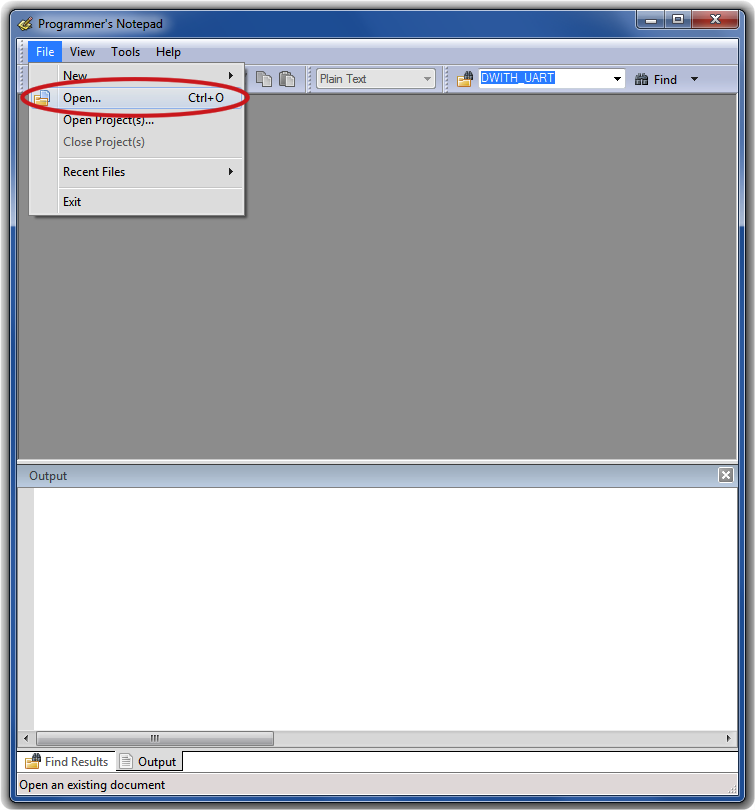
\includegraphics[width=9cm]{../PNG/Notepad_open.png}
    \caption{open Makefile}
  \end{subfigure}
  ~
  \begin{subfigure}[b]{9cm}
    \centering
    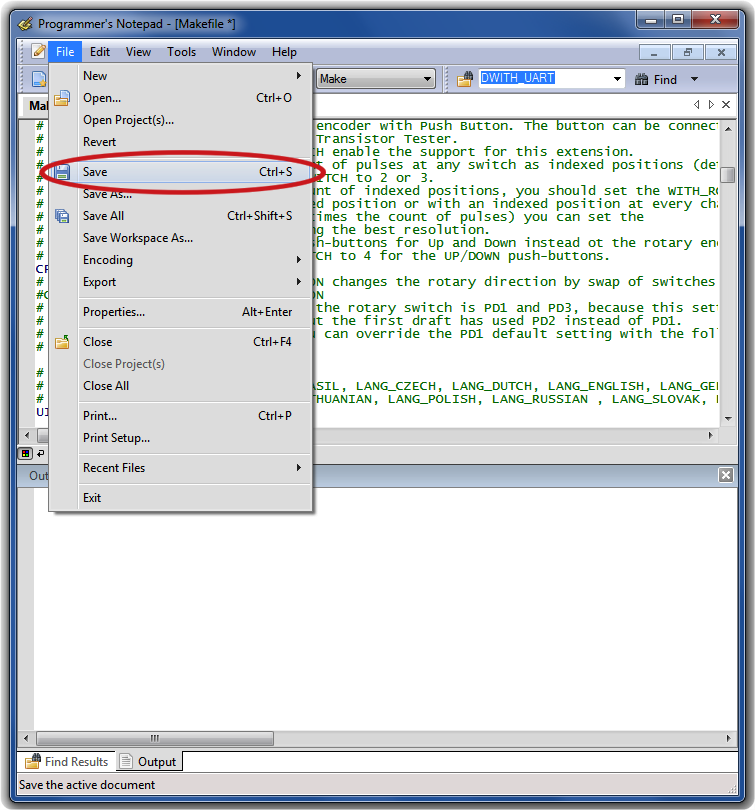
\includegraphics[width=9cm]{../PNG/Notepad_save.png}
    \caption{save Makefile}
  \end{subfigure}
  \caption{Bedienung der WinAVR-Oberfläche Programmer's Notepad}
  \label{fig:WinAVR1}
\end{figure}

Die nächsten Abbildungen \ref{fig:WinAVR2} zeigen das Tools-Menü von Programmer's Notepad
zum Übersetzen des Programms (Make All) und zum Programmieren des ATmega (Program) mit avrdude.

\begin{figure}[H]
  \begin{subfigure}[b]{9cm}
    \centering
    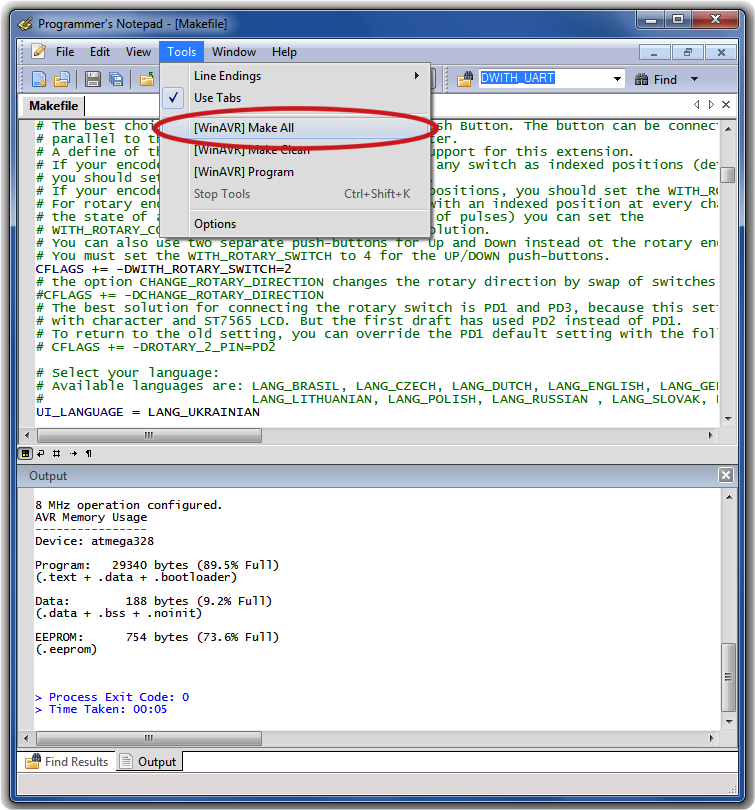
\includegraphics[width=9cm]{../PNG/Notepad_make.png}
    \caption{Erzeuge Programmdaten (.hex/.eep)}
  \end{subfigure}
  ~
  \begin{subfigure}[b]{9cm}
    \centering
    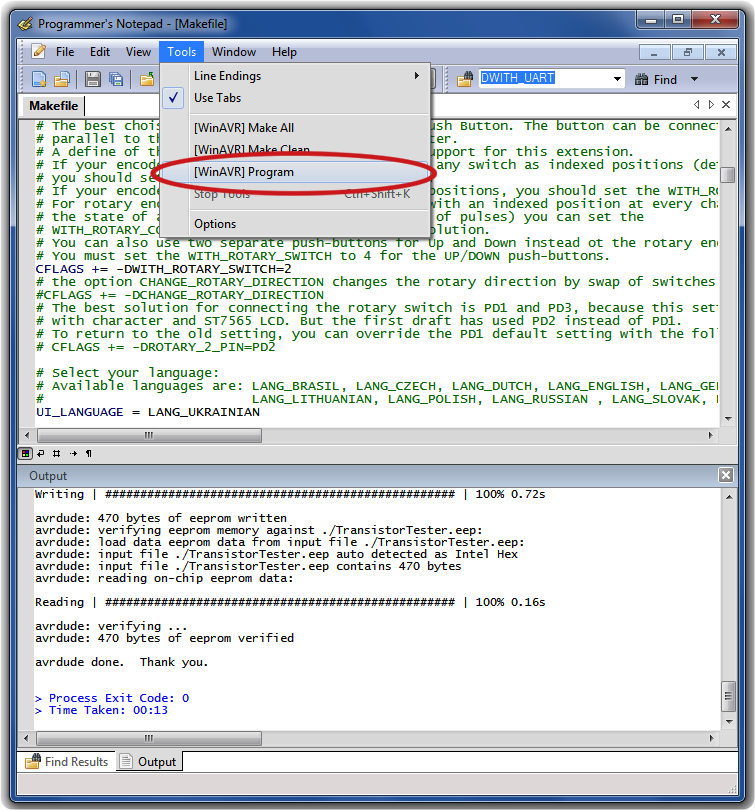
\includegraphics[width=9cm]{../PNG/Notepad_program.png}
    \caption{Programmiere ATmega}
  \end{subfigure}
  \caption{Bedienung der WinAVR-Oberfläche Programmer's Notepad}
  \label{fig:WinAVR2}
\end{figure}


\section{Fehlersuche}
Bei den meisten Problemen werden Sie den Text auf dem LCD-Display vermissen.
Zuerst sollten Sie prüfen, ob die LED auf der Platine schwach leuchtet, wenn Sie den Start-Taster
loslassen.
\begin{description}

\item[Gerät schaltet nicht ein]  
Wenn die LED nicht leuchtet, aber die VCC-Spannung den richtigen Wert hat, wenn
man den Start-Taster gedückt hält, schaltet der Mikrocontroller nicht richtig ein.
Der Mikrocontroller sollte die Spannung behalten indem der Ausgang PD6 auf \(5V\)
geschaltet wird, was üblicherweise als eine der ersten Aktionen getan wird.
Wenn man die Start-Taste gedrückt hält, bleibt die Spannung ohnehin eingeschaltet.
So können Sie mit gedrücktem Taster den Wert der VCC-Spannung und zusätzlich den Spannungswert am
Ausgang PD6 prüfen.
Wenn die VCC-Spannung den richtigen Wert (\(5V\)) hat, aber die Spannung am Ausgang
PD6 unter \(4V\) ist, startet der Mikrocontroller nicht richtig.
Für diesen Fall sollten Sie prüfen, ob die Programmdaten für den Flashspeicher
für den richtigen Prozessor-Typ ist und ob der Prozessor richtig konfiguriert ist (fuses).
Wenn der ATmega den Ausgang PD6 auf \(5V\) schaltet und die Betriebsspannung 
trotzdem nicht eingeschaltet bleibt, wenn man den Start-Taster loslässt, ist der
Grund schwieriger zu finden.
Zuerst kann man die LED kurzschliessen und es noch einmal versuchen.
Wenn der Tester jetzt startet, ist die LED möglicherweise falsch herum eingebaut.
Wenn das nicht die Ursache ist, könnte der Grund ein unzureichender Stromverstärkungs-Faktor
des Transistors T3 (BC557C) sein.
Der Strom in die Basis von T3 ist niedriger, wenn der Mikrocontroller mit der LED einschaltet
wie im ,,Taster gedrückt''-Zustand.

\item[Nichts ist lesbar auf der LCD-Anzeige] 
Prüfen Sie die Spannung am Kontrast-Pin der LCD-Anzeige (Pin 3).
Stellen Sie mit dem Trimmer den Wert auf einen im Datenblatt angegebenen Wert und optimieren Sie
durch Sichtkontrolle.
Wenn Sie ein Hochtemperatur-Display haben, brauchen Sie eine negative Kontrast-Spannung für
den Betrieb.
In diesem Fall kann man den ICL~7660-Baustein zum Erzeugen der negativen Spannung aus der
positiven \(5V\) verwenden.

Der Tester kann für viele verschiedene Controller mit unterschiedlichen Anschlußarten
konfiguriert werden. Prüfen sie auf jeden Fall, ob die Software zu ihrem Display paßt.
Wenn keine Anzeige auf dem LCD erkannt wird und wenn die Hintergrundbeleuchtung an ist,
sollten Sie die Spannungsversorgung trennen und alle vier Datenverbindungen sowie die 
beiden Steuersignale überprüfen.
Wenn alle Verbindungen in Ordnung sind, sehe ich als Ursache nur noch die Möglichkeit einer
falschen Zeitabfolge der Steuersignale.
Die Ursache hierfür kann sein, dass der LCD-Controller langsamer ist als es die Software
des ATmega erwartet. Es könnte auch sein, dass der ATmega auf der falschen Taktrate läuft.
Bitte überprüfen Sie für welche Taktrate die Software übersetzt ist und ob
die fuses des ATmega für diese Geschwindigkeit richtig gesetzt sind.
Sie finden die eingestellte Taktrate in der betreffenden Makefile.
Wenn der Tester ohne die Abschalt-Elektronik aufgebaut ist, kann man mit einer
an die Test Pins angeschlossenen LED testen, ob das Programm arbeitet.
Wenn die LED flackert, läuft das Programm. Der Fehler muss in diesen Fall an
dem Anschluss des LCD's liegen. 
Bei einigen graphischen Displays kann der Kontrast über eine Menüfunktion verstellt werden.
Wenn man hier versehentlich den Kontrast zu weit verstellt hat, ist auf dem Display
nicht mehr zu erkennen, man kann also auch nicht mehr weiter bedienen.
Hier können Sie nur versuchen, ob von der Seite (schräg) doch noch etwas zu erkennen ist
und über das Menü den Kontrast zurückstellen. Wenn dan nicht geht, können sie
das EEprom des ATmega mit einem ISP programmer neu beschreiben und damit den Kontastwert zurückstellen.
\item[Einiges, aber nicht alles ist auf der LCD-Anzeige lesbar] 
Überprüfen Sie ob die .eep-Daten in den EEPROM des ATmega geladen wurden.
Wenn alle Programmdaten richtig geladen wurden, sollten Sie die Taktrate ihrer
Programmdaten (Makefile) und die ATmega-Einstellungen prüfen (fuses).

\item[Messung ist zu langsam und Kapazitäten werden um Faktor 8 zu klein gemessen.] 
Sie betreiben die Software, die für \(8MHz\) übersetzt wurde mit einer Taktrate von \(1MHz\).
Bitte konfigurieren Sie den ATmega mit den fuses richtig.

\item[Die Messung ergibt seltsame Ergebnisse]  
Überprüfe ob der ISP-Programmierstecker noch verbunden ist.
Der ISP-Stecker sollte nicht während einer Messung eingesteckt bleiben.
Sehr oft ist der Grund für falsche Messergebnisse, dass die Software mit der
 AUTOSCALE\_ADC Option und der NO\_REF\_CAP Option übersetzt wurde, aber der
Kondensator am AREF-Pin hat immer noch einen Wert von \(100nF\).
Falsche Bestückung von Bauteilen können auch eine Ursache für Messfehler sein 
oder zurückgebliebene Flussmittelreste können die Messung stören.
Bitte prüfen Sie nach Möglichkeit mit der Selbsttest-Funktion der
TransistorTester-Software.
Zu den Einzelheiten schauen Sie in das Selbsttest-Kapitel \ref{sec:selftest}.

Anderenfalls prüfen sie Ihre Platine visuell und prüfen Sie die Widerstandswerte
mit einem Ohmmeter. Sie können die Pins des ATmega für diese Prüfung benutzen,
zum Beispiel können Sie der Widerstand R1 zwischen Pin 23 und Pin 14 messen.
Schauen Sie in das Schaltbild \ref{fig:ttester} für die Einzelheiten.
Man braucht den Mikrocontroller nicht zu entfernen, nur die Stromversorgung sollte
vorher getrennt werden.

\item[Der Tester schaltet nach 2 Sekunden Anzeigezeit aus]  
Dies ist dann der Fall, wenn der Pull-Up-Widerstand am PD7-Eingang
fehlt oder der Taster dauernd gedrückt wird. 
Die Software schaltet die internen Pull-Up-Widerstände ab, um eine Beeinflussung
der Messergebnisse auszuschließen. Deswegen ist ein externer Widerstand erforderlich.

\item[Der Tester zeigt immer nur Vext=xx.xV in Zeile 2 an]
Dies ist dann der Fall, wenn der Pull-Up-Widerstand am PD7 Eingang
fehlt oder der Taster dauernd gedrückt wird.
Die Software ist außerdem ohne seriellen Ausgang (ohne Option WITH\_UART) und
ohne interne Pull-Up Widerstände (mit Option PULLUP\_DISABLE) konfiguriert.
Installieren Sie einen Pull-Up Widerstand an PD7.

\end{description}
